%% Sample dissertation using the kau_report LaTeX class
%%
%% 950203  Michael Kelsey -- LaTeX2e format (cit_thesis)
%% 990210  Anna Brunstrom -- Modified to KAU requirements
%% 990420  Anna Brunstrom -- Copyright page added + some minor updates

%\documentclass{kaumasters}
\documentclass[12pt,twoside]{kau_report}

\usepackage{float}
\PassOptionsToPackage{hyphens}{url}\usepackage{hyperref}
\usepackage{url}
\usepackage{subfig}
\usepackage{tabularx}
\usepackage{listings}
\usepackage{color}
\usepackage{pdfpages}
\usepackage{mathtools}
\usepackage{chngcntr}
%\usepackage{refcheck}

\newcommand{\itab}[1]{\hspace{0em}\rlap{#1}}
\newcommand{\tab}[1]{\hspace{.2\textwidth}\rlap{#1}}

\AtBeginDocument{\counterwithin{lstlisting}{section}}

\setlength{\fboxsep}{0pt}

\definecolor{dkgreen}{rgb}{0, 0.6, 0}
\definecolor{gray}{rgb}{0.5, 0.5, 0.5}
\definecolor{mauve}{rgb}{0.58, 0, 0.82}
\lstset
{
	frame=tb,
	aboveskip=3mm,
	belowskip=3mm,
	showstringspaces=false,
	columns=flexible,
	basicstyle={\small\ttfamily},
	numbers=left,
	numberstyle=\color{gray},
	keywordstyle=\color{blue},
	commentstyle=\color{dkgreen},
	stringstyle=\color{mauve},
	breaklines=true,
	breakatwhitespace=true,
	tabsize=3,
}

% If you write in Swedish, uncomment line below
%\usepackage{swedish}

% Define the parameters in the preamble

\title{An Evaluation of Google Glass\\ 
\large Design, Implementation and Evaluation of an Product Assembly Application for Google Glass and Smartphones}
%\swetitle{En Utv{\"a}rdering av Google Glass\\ 
%\large Design, Implementation and Utv{\"a}rdering av en Produktsammans{\"a}ttningsapplikation f{\H o}r Google Glass och Smarttelefoner}

%\swetitle{En Utvärdering av Google Glass\\ 
%\large Design, Implementation and Utvärdering av en Produktsammansättningsapplikation för Google Glass och Smarttelefoner}


\pubnum{June, 2015}
%\swepubnum{Juni, 2015}

\author{Johan H\"{a}ger}

\date{2015-06-05}

\advisor{Donald F. Ross}
\examiner{Thijs. J. Holleboom}

% The actual document starts here
\begin{document}


% Create the title page. If you write in swedish use the second
% line below instead.
\makekautitle
%\newpage
%\newpage
\makeswekautitle

%% Create the copyright page. If you write in swedish use the second
% line below instead.
\copyrightpage
%\swecopyrightpage

 %Start roman numbering
\begin{frontmatter}

% Create approval page. select the appropriate command depending
% on how many authors you have. If you write in swedish use 
% one of the sweapproved lines below instead.
%\approved
\approved
%\approvedthree{Author One}{Author Two}{Author Three}
%\sweapproved
%\sweapprovedtwo{Author One}{Author Two}
%\sweapprovedthree{Author One}{Author Two}{Author Three}

% Create abstract 
\begin{abstract}
Assembling components in a production line could potentially be a tedious task, if performed stepwise by the book. However, an employee who is assembling many different products may not know all the steps by heart. As such they will be reliant on an instruction manual. However, an instruction manual must be carried around and, while assembling components, placed in the assembler's line of sight. Instead new technology could make the process more efficient. Google Glass places a display slightly above the user's line of sight and can be controlled via voice commands, and as such solves many of the problems associated with carrying around instruction manuals. This dissertation is an evaluation of Google Glass and describes the design, implementation and evaluation of an product assembly application for both Google Glass and smartphones. The smartphone version was implemented in order to provide a reference point as well as means of comparison with the Google Glass application. The test application used in the study was to read a QR code and download a set of assembly instructions. Testing was carried out on the different steps of the application, from when the QR code has been scanned until the information was displayed to the user. The results show that Google Glass is almost always slower, in all steps, compared to the smartphone equivalents. The conclusion is that Google must upgrade and improve on Google Glass and in particular the hardware. Google Glass overheats easily and the camera is of inferior quality. Google's implementation restrictions also limits what developers might be able to do with the device. However, Google Glass is easy to use and has potential to become a more useful device in the future.
\\
% KEYWORDS
\\
\textbf{Keywords:} Google Glass, Android, Front-end, Performance evaluation
%Motivation:
%Why do we care about the problem and the results? If the problem isn't obviously "interesting" it might be better to put motivation first; but if your work is incremental progress on a problem that is widely recognized as important, then it is probably better to put the problem statement first to indicate which piece of the larger problem you are breaking off to work on. This section should include the importance of your work, the difficulty of the area, and the impact it might have if successful.
%Problem statement:
%What problem are you trying to solve? What is the scope of your work (a generalized approach, or for a specific situation)? Be careful not to use too much jargon. In some cases it is appropriate to put the problem statement before the motivation, but usually this only works if most readers already understand why the problem is important.
%Approach:
%How did you go about solving or making progress on the problem? Did you use simulation, analytic models, prototype construction, or analysis of field data for an actual product? What was the extent of your work (did you look at one application program or a hundred programs in twenty different programming languages?) What important variables did you control, ignore, or measure?
%Results:
%What's the answer? Specifically, most good computer architecture papers conclude that something is so many percent faster, cheaper, smaller, or otherwise better than something else. Put the result there, in numbers. Avoid vague, hand-waving results such as "very", "small", or "significant." If you must be vague, you are only given license to do so when you can talk about orders-of-magnitude improvement. There is a tension here in that you should not provide numbers that can be easily misinterpreted, but on the other hand you don't have room for all the caveats.
%Conclusions:
%What are the implications of your answer? Is it going to change the world (unlikely), be a significant "win", be a nice hack, or simply serve as a road sign indicating that this path is a waste of time (all of the previous results are useful). Are your results general, potentially generalizable, or specific to a particular case?

\end{abstract}
\cleardoublepage


% If you write in swedish you need a second abstract in 
% English. Uncomment lines below for the second absract.
\renewcommand{\abstractname}{Abstract (In Swedish)}
\begin{abstract}

Montering av komponenter i en produktionslinje kan potentiellt vara en tradig och mekanisk uppgift, om det utf{\H o}rs stegvis enligt instruktioner. En anst{\"a}lld som bygger m{\aa}nga olika produkter kan dock eventuellt inte samtliga steg utantill, utan blir beroende av en bruksanvisning. En bruksanvisning m{\aa}ste dock b{\"a}ras runt och, vid montering av komponenter, l{\"a}mnad i monterarens siktlinje. Ny teknik skulle kunna g{\H o}ra processen mer effektiv. Google Glass heter den enhet som placerar en display n{\aa}got {\H o}ver anv{\"a}ndarens siktlinje och kan styras via r{\H o}stkommandon, och s{\aa}ledes l{\H o}ser m{\aa}nga av de problem som {\"a}r f{\H o}rknippade med att b{\"a}ra runt en bruksanvisning. Denna uppsats {\"a}r en utv{\"a}rdering av Google Glass och beskriver utformning, implementering och utv{\"a}rdering av en produktsammansättningsapplikation f{\H o}r b{\aa}de Google Glass och smarttelefoner. Smarttelefon-versionen implementerades i syfte att ge en referenspunkt samt medel f{\H o}r j{\"a}mf{\H o}relse med Google Glass applikationen. Test-applikationen som anv{\"a}nds i studien kan skanna en QR-kod och ladda ner en upps{\"a}ttning monteringsanvisningar. Testning utf{\H o}rdes p{\aa} de olika stegen i applikationen, fr{\aa}n n{\"a}r QR-koden har skannats tills informationen visas f{\H o}r anv{\"a}ndaren. Resultaten visar att Google Glass n{\"a}stan alltid {\"a}r l{\aa}ngsammare, i alla steg, j{\"a}mf{\H o}rt med smarttelefon-ekvivalenter. Slutsatsen {\"a}r att Google m{\aa}ste uppgradera och f{\H o}rb{\"a}ttra Google Glass, och s{\"a}rskilt h{\aa}rdvaran. Google Glass {\H o}verhettas l{\"a}tt och kameran {\"a}r av s{\"a}mre kvalitet. Googles implementationsbegr{\"a}nsningar begr{\"a}nsar ocks{\aa} vad utvecklarna skulle kunna g{\H o}ra med enheten. Google Glass {\"a}r dock l{\"a}tt att anv{\"a}nda och har potential att bli en mer anv{\"a}ndbar enhet i framtiden.
\\
% NYCEKLORD
\\
\textbf{Nyckelord:} Google Glass, Android, Front-end, Utv{\"a}rdering av prestanda

\end{abstract}
\cleardoublepage

% Create acknowledgements (optional part)
\begin{acknowledgements}
Firstly, I would like to thank Richard Hoorn, who has been my partner in crime on this project. Without your amazing work on the back-end part of the project, my work on the front-end would simply be half the solution to the original problem.

I would also like to send a big thank you to Donald F. Ross at Karlstad University for being my supervisor throught the writing of this dissertation, for always pushing me forward and inspiring me to do even better.

Also at Karlstad University, I would like to thank Daniel Johansson, laboratory engineer at Karlstad University, for allowing me to borrow the equipment used in the experimental setup.

I would like to thank Mats Persson at Sogeti, Karlstad, for being my supervisor during the development process and making sure the project stayed on track, with feedback and check-ups during regular sprint demonstrations. 

Thank you also to Kalle Henriksson at Sogeti Karlstad, for taking your time to help review the code and for coming with useful tips and tricks on how the code could be improved.

Thank you to Sogeti Karlstad, overall, for allowing me to take on such an interesting project and for allowing me to work with such exciting, new technology. 

Also a big thank you overall to all the people over at Sogeti Karlstad for always making me feel welcome and for all the good chats and talks over breaks and lunches.

Finally, thank you to all those who have wished me good luck, or in any other way supported me throughout working on this project. Your kind words means a lot!

% I would like to thank my supervisor at Karlstad University, Donald F. Ross, for 
%Mats Persson - handledare Sogeti sprintdemo

%Donald F. Ross - handledare kau

%Kalle Henriksson - kodgranskning

%Daniel Johansson - utlåning av testequipment kau

% Richard Hoorn second part of project

%Sogeti i allmänhet

%A final thank you to everyone who have been supportive and wished me good luck throughout the process of working on this project as well as writing this dissertation.

% If you want acknowledgements they go here 
\end{acknowledgements}
\cleardoublepage

% Set up contents, list of figures and list of tables
  \tableofcontents
  \cleardoublepage

  \listoffigures
  \cleardoublepage

  \listoftables
  \cleardoublepage
  
  \lstlistoflistings
  \cleardoublepage

\end{frontmatter}
% End of roman numbering

% Here comes the main body, it's your job to fill this in...
\section{Introduction}
\label{sec:introduction}
%o   Project goal and motivation
%o   Project summary and overview - the "red thread"
%o   Project results (brief summary)
%o   Dissertation Layout
%
%Nytta med projektet, bakomliggande motivering, hypotes kring resultat (Google Glass kommer vara bättre än smartphone eftersom handsfree and stuff), layout av rapporten.
%
%Prata allmänt om vad det finns för problem idag, mer specifikt vad kommer vår applikation att lösa, mixa med frågor som kan besvaras bland slutsatserna
%
%
%
todo sogeti ska med?

todo acknowledgments

Although assembling components in to a fully functional product can be a tedious task and done by the books, step-by-step, an employee constructing many different products may not be able to learn the process by heart, and will need to rely on instruction manuals.

However, carrying instruction manuals around would mean having to find specific instruction and also, while assembling components, the instructions will have to be laid aside. As such, the constructor's focus will have to shift between the components and the instructions, perhaps turn the head around, and potentially the constructor may even need to use their hands in order to browse the instructions. 

Using a smartphone at least removes the requirement for written instructions on paper, but a smartphone still requires touch and as such will occupy at least one of the constructor's hands at some point. A smartphone, similar to ring binders, will also have to be laid aside.

One solution to the problem would be using a TV or computer screen. Controlled with for instance foot pedals the instructions could be browsed without using hands. However, such technology requires space and also comes with the fact that such technology is not very mobile. Screens and foot pedals would have to be positioned at specific locations. Considering a production line may have several stations screens and foot pedals would have to be placed at each one of them. Trying to assemble components outside of those stations would not be possible, provided that the instructions would be necessary.

New technology may offer a better solution. Google Glass is a computational device, which looks and is worn as regular glass frames~\cite{glassStart}. Google Glass also has a display positioned slightly above the user's line of sight, meaning that Google Glass does not have to be taken off and put down. Google Glass may also be entirely controlled via voice commands, meaning that the user may operate Google Glass completely hands free.

This dissertation describes the design, implementation and evaluation of an application for Google Glass. Using the application, user's will be able to scan a QR code related to a specific product and get information on which components are needed to construct the specific product, as well as instructions on how to assemble the components.

The application will also be built for smartphones, giving a reference point for the evaluation as well as a method of comparison with the Google Glass application. Using the Google Glass application users will be able to construct products by following instructions, but without having to shift their focus from what they are doing, and neither will the users have to use their hands in order to control the application.

\subsection{Discontinuance of the Explorer Program}
It should be noted that, since the start of this dissertation, Google have chosen to cancelled the so called ``explorer program'' for Google Glass~\cite{glassDiscontinued}. The explorer program was the ``open beta phase'' of Google Glass where Google, although Google Glass was sold as a consumer product, were still developing Google Glass at Google's research center, called Google X. Google used user's input and feedback to improve on Google Glass as a product, both in terms of hardware as well as software.

Coming out of the open beta phase, Google have now chosen to keep developing Google Glass, but without the help of consumers, meaning that any further updates, both in terms of hardware as well as software, will (as of now) not be publicly available. Google states that they are ``thrilled to be moving even more from concept to reality'', when discussing the future of Google Glass. As of January 20th, 2015, the Google Glass Explorer Edition was no longer available for sale. However, Google ensures that Google Glass will return ``when they're ready'', but does not go in to further details on when Google Glass will be available for sale again or what the new version will entail. 

\subsection{Back End}
todo

\subsection{Hypothesis}
The hypothesis is that the Google Glass application will prove useful and valuable, more so than the smartphone application. Although Google Glass might not be the most powerful device on the market, the features of Google Glass are the selling points. 



Google Glass should at least be close enough to the smartphone in terms of performance, giving weight to the argument that Google Glass should be used in order to make the assembling of components an easier task.

todo redo, back up statements with facts. What is expected and why? How should the results be interpreted if they show the expected?

\subsection{Project Results}
The results show that Google Glass is almost always slower, both in terms of decoding the QR code and presenting the information to the user. On average Google Glass is about half a second slower than smartphone equivalents. In terms of the amount of information that may be displayed on the Google Glass display compared to the display on smartphones it was shown that the same amount of text that filled the screen on a smartphone needed three to four separate screens on Google Glass.

\subsection{Dissertation Layout}
Chapter~\ref{sec:background} discuss relevant background information regarding Google Glass. The chapter will include an introduction to what Google Glass is, how they came about and what features they have. The background chapter will also discuss similar products to Google Glass, as well as compare Google Glass to smartphones. Finally chapter two will include some discussion on topics relevant to the project, including QR code and ways of presenting information.

Chapter~\ref{sec:design} is about the design of the project. The discussion revolves around how the application is intended to work, and what limitations may apply to the implementation of the application, both on Google Glass and smartphone. The third chapter also discusses the design of the tests done on the application.

Chapter~\ref{sec:implementation} describes the implementation part of the project. The flow of the application is described in detail. Specific aspect of the application is also described in more detail. The layout of the slides as well as the voice commands. The experimental setup and how the tests were performed is also described here.

In chapter~\ref{sec:resultevaluation} the results of the tests are presented. The results are presented along with comments regarding how the results are to be interpreted as well as comments on any potential error factors during testing.

The final chapter, chapter~\ref{sec:conclusion}, contains conclusions on the project. The conclusions regards the test results, as well as conclusions on the project as a whole. Chapter six also includes comments based on personal user experience from using Google Glass for about three months. Finally future work is discussed and the report is concluded with some concluding remarks.

Attached to the dissertation, after the reference list, are appendices. In appendix~\ref{sec:abbreviations} abbreviations used throughout the dissertation are listed. Appendix~\ref{app:results} shows all the individual test results. Project code can be found in appendix~\ref{app:code}. Appendix~\ref{app:projectspec} is the last appendix which contains the original project specification, written in Swedish.
\cleardoublepage

\section{Background}
\label{sec:background}
%How did Google Glass come about? History!
%Mobiles today are used as a nervous tick. It is a distraction and something that pulls your attention away from the real world. At least that is what Sergey Brin, one of the founders of Google, claimed during a Ted Talk presentation in February 2013.\cite{tedtalkWhyGlass} Brin stated that if he was a smoker he would probably light a cigarette at those times when he now uses his phone.
%\url{http://www.ted.com/talks/sergey_brin_why_google_glass}
%
%Brin and his team wanted to create something that would make interaction with technology easy and fast and not distract from reality. They wanted to keep the information more handy and close by than a phone stuck in the users pocket. But they also wanted to keep the line of sight free. Thad Starner, technical lead/manager on Google Glass, wrote in an article in 2013,\cite{6504855} that he sought out to build something as intuitive as a watch. An extension of the self, as he stated. And so Google started working on Project Glass. 
%
%
%
%
% The idea behind Glass was to minimise the time between intention and action
% users should not have to bring up something from their pockets each time they want to interact with technology
% they should be able to just simply interact
% They wanted to create something as intuitive as a watch. 
% checking the watch is something a user might do without actually thinking about what the time is.
% they might have to check again if someone were to ask them what the time is.
% Glass should be an extension of the self rather than another device.
% // Thad Starner - technical lead/manager on Google Glass
%
% Sergey Brin, one of the founders at Google, has similar ideas
% ted talk he spoke about how checking the phone was something he did without reason
% putting notifications more easily accessible would minimise interaction with technology because the user
% would not have to check if any updates have come in, they would know right away
%
%
On April 4th, 2012, Google announced ``Project Glass''.\cite{GoogleGlassConcept} Google Glass, as the device is now known, was under development for several years at Google's research and development department, Google X. As part of the announcement Google stated:  ``We think technology should work for you---to be there when you need it and get out of your way when you don't.''.\cite{GoogleGlassAnnouncement}

Serge Brin, one of the founders of Google, gave a Ted Talk in February 2013\cite{tedtalkWhyGlass} where he talked about why Google decided to produce the device. His argument was that users stayed on their smartphones for too long. Brin also argued that when users were using their smartphones they were looking down on a screen and were not aware of their surroundings. Instead Google wanted to create a device that would give the user notifications that could quickly be dealt and done with. Google also wanted to make the device hands-free and put the display where the user did not have to look down. Brin stated that the development team at Google X added the camera later on in the development process but that the camera had been a great addition to the device and enabled Google Glass to capture the user's surroundings, for instance by taking photographs.

Thad Starner, technical lead/manager on Google Glass, claimed that Google Glass was supposed to be an extension of the self.\cite{6504855} He compared Google Glass to a watch. Not in terms of where the user keeps his or her focus (with a watch you must look down, similar to a smartphone), but rather in terms of how a watch is easy to access and how the access is instant. Starner said that with Google Glass, Google wanted to minimise the time between intention and action. 
%
\subsection{What is Google Glass?}
\label{subsec:googleglass}
Google Glass, or simply Glass as the device is known within Google, is a head mounted display (HMD) that can be seen as an augmented reality device\footnote{See section \ref{subsubsec:augmentedrealityvsvirtualreality}} designed to bring notifications to the user more easily than a smartphone does. According to Google ``Glass is designed to be there when the user needs it and to stay out of the way when the user does not''.\cite{glassDesignPrinciples} Google Glass is meant to give the user relevant information at relevant times.\\ 
%\url{https://developers.google.com/glass/design/principles}

Google Glass is partially controlled via a touchpad (it can also be controlled with voice command). The touchpad sits on the right hand side of the user's glass frame and runs from the temple to the ear. When the user touches anywhere on the touchpad Google Glass ``wakes up'' from stand by and displays the start screen (which consists of a clock). The display is mounted above the user's line of sight, on the right hand side. The display can be slightly adjusted so that the user can see everything displayed. \\







	\begin{figure}[ht!]
		\centering
		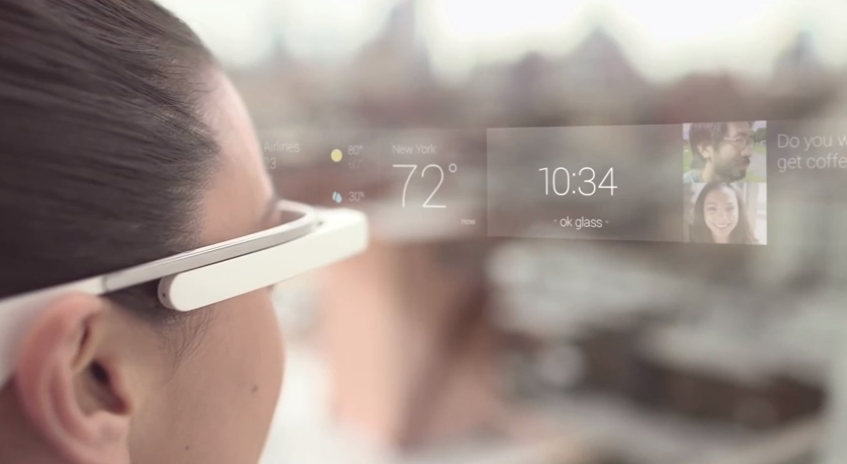
\includegraphics[width=110mm]{images/GoogleGlassUI}
		\caption{A virtual representation of the Google Glass user interface as the graphical user interface is perceived by the user.\cite{ImagesGoogleGlassUI}}
		\label{GoogleGlassUI}
	\end{figure}
	
	
	




The graphical user interface (GUI) is called a timeline (see Figure \ref{GoogleGlassUI}). The timeline consists of a row of cards. Cards are basic applications such as a clock or information about the weather. Cards can also represent more in-depth applications, on Google Glass called ``Immersions''. An immersion handles activities such as browsing an image gallery or playing a game.\\

On the timeline cards to the left of the home screen are upcoming activities such as an event in the user's calendar or an upcoming flight. Cards to the right of the home screen are from the past. Cards from the past will for instance show text messages or photos. When the user wants to turn of Google Glass the user swipes down on the touchpad. Swiping down on the touchpad will put Google Glass in stand by. If the user wants to turn of Google Glass entirely there is a power button on the opposite side of the touchpad. Holding down the power button for a few seconds will turn of Google Glass. For a better visual understanding of how Google Glass works see Figure \ref{GoogleGlassUI} as well as the video referenced in the caption.\\

%Glass uses a small display placed to the upper right of the user's line of sight and is mounted on the user as a regular pair of glasses. Equipped with a camera, microphone and speakers it is capable of performing a lot of the tasks users normally would do on a smartphone such as taking photographs, video chatting, writing text messages.

The principles behind designing for glass is to keep the information relevant. Google ranks different computational devices and services in terms of time periods. Google talks about how the cloud stores information ``forever'', a computer keeps about a years worth of information, a mobile phone is keeping track of the last month and Glass are for the present.

Therefore Google asks developers to keep the information relevant and simple. Glass is designed not to get in the way of the user and, as stated previously, be usable when the users wants to.\cite{glassDesignPrinciples}
%\url{https://developers.google.com/glass/design/principles}

\subsubsection{Augmented Reality vs Virtual Reality}
\label{subsubsec:augmentedrealityvsvirtualreality}

[TODO WRITE ABOUT HUD AND HMD]

When discussing head mounted displays it is possible that the first image that pops into ones head is similar to Figure \ref{OculusRift}. What is important to note about Oculus Rift (Figure \ref{OculusRift}) and other similar product that completely covers the user's eyes is that these are all virtual reality devices. Virtual reality is not the same as augmented reality, which is what Google Glass gives the user.



	\begin{figure}[ht!]
		\centering
		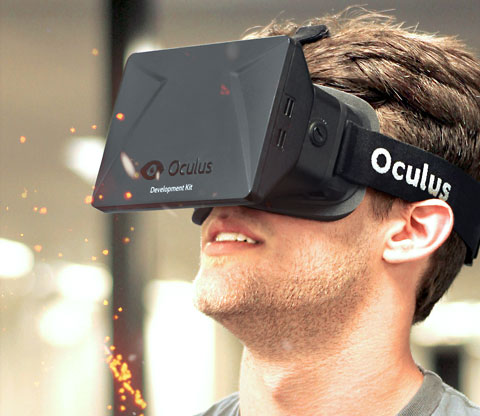
\includegraphics[width=110mm]{images/OculusRift}
		\caption{The virtual reality device Oculus Rift is a head mounted display that covers the user's eyes completely\cite{ImagesOculusRift}}
		\label{OculusRift}
	\end{figure}





The difference lies in how much of what the user can see is computer generated. In a virtual reality the entire environment is computer generated. Augmented reality on the other hand is based in reality where computer generated elements of the environment help enhance reality. In other words: virtual reality replaces reality and augmented reality enhance reality. Since Google Glass does not remove the user from reality but rather display information that can be consumed at the same time as the user experience the real world Google Glass is an augmented reality device compared to Oculus Rift which is a virtual reality device.

TODO --- ADD HUD vs AUGMENTED REALITY!!!!!!


%What is it?
%Augmented Reality vs Virtual Reality
%Define Augmented Reality
%Define Virtual Reality

%
\subsection{Similar Products}
\label{subsec:similarproducts}
Today there are several products, either already on the market or under development, that are more or less similar to Google Glass. The following is a short list (a more extensive list of devices can be found on Wikipedia~\cite{ohmdWiki}) describing some of the competition Google Glass faces, with each product shown in Figure ~\ref{imagesSimilarProducts}. 

	\begin{figure}[H]%ht!]
		\centering
    	\subfloat[Microsoft Hololens~\cite{hololens}]{{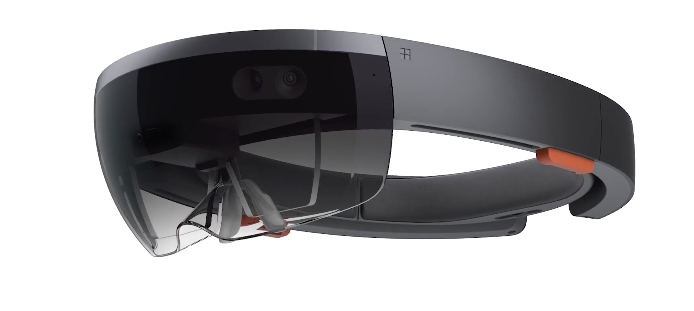
\includegraphics[width=70mm]{images/similarProducts/hololens}}}
    \qquad
    	\subfloat[Recon Jet~\cite{reconJet}]{{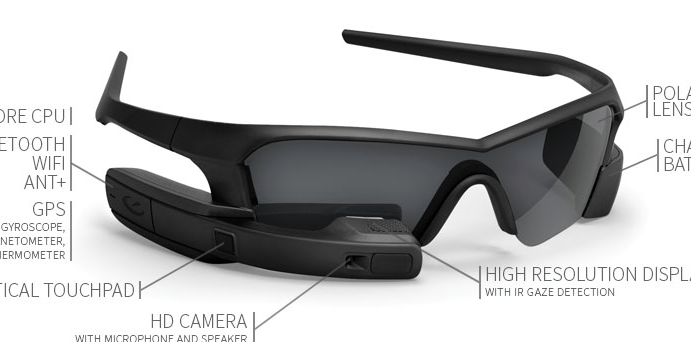
\includegraphics[width=70mm]{images/similarProducts/reconJet}}}
    \qquad
        \subfloat[GlassUp~\cite{glassUpFeatures}]{{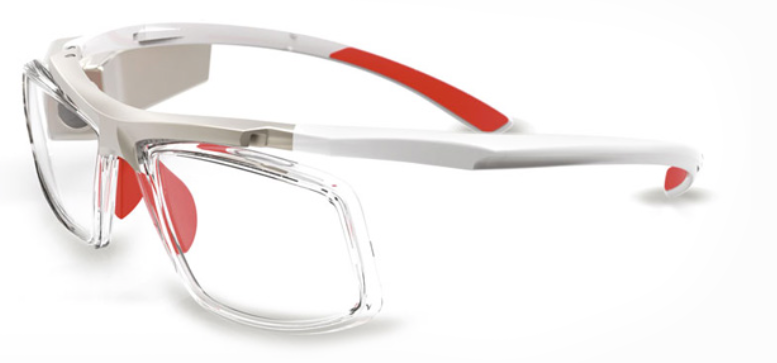
\includegraphics[width=70mm]{images/similarProducts/glassUp}}}
    \qquad
  	\subfloat[C Wear Interactive Glasses~\cite{pennyProducts}]{{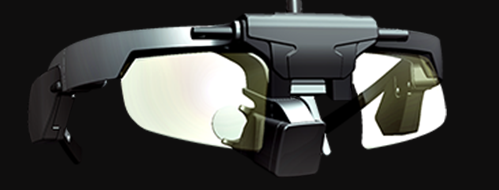
\includegraphics[width=70mm]{images/similarProducts/penny}}}
    \qquad
		\caption{There are many OHMD devices similar to Google Glass~\cite{ohmdWiki}.}
		\label{imagesSimilarProducts}
	\end{figure}
	

\subsubsection{Microsoft Hololens}

Microsoft's offer in the augmented reality device space is an HUD that displays information in front of both of the user's eyes. Microsoft's device is called Microsoft Hololens and can be seen in Figure~\ref{imagesSimilarProducts}~(a)~\cite{hololens}. 
%The intention, according to Microsoft, is not to be an immediate competitor to Google Glass. Microsoft's aim is not to make the same device as Google Glass. 
While Google Glass is meant to be worn at all times, Microsoft Hololens is rather a device users only wear when they intend to use Microsoft Hololens. Google Glass is, as Thad Starner stated~\cite{6504855}, meant to be an extension of the self and is meant to be worn at all times, even though the user might not be actively using Google Glass at the time, in order to bring helpful notifications and information to the user. Microsoft Hololens is rather a tool to be used actively for a certain purpose, such as modelling~\cite{hololensDemo}, and then put away. Google Glass may be used the same way if the user wants to, but that is not the intent.

The mot striking difference between Microsoft Hololens and Google Glass lies in the interaction with the real world. Google Glass is a two-dimensional (2D) display that sits slightly above the users line of sight% (see Section~\ref{subsec:googleglass})
. Microsoft Hololens, on the other hand, is meant to interact with the world even further.

Microsoft intends to give the user tools to work in a 3D space. Microsoft's concept video~\cite{hololensConceptVideo} of Microsoft Hololens shows examples of 3D modelling with the use of kinetic hand-movement detection. Microsoft Hololens will enable users to see what they are working on from different angles simply by walking around the object, just as if the object in question were real and had a physical mass.

\subsubsection{Recon Jet}

Recon Jet, seen in Figure~\ref{imagesSimilarProducts}~(b), is an HMD developed by Recon Instruments~\cite{reconJet}. Recon Jet is suited for athletes. Because of the target audience, Recon Jet has been fitted with a display that has high contrast in order to give good readability in high ambient lighting. The display's virtual image appears as  a 30 inch wide screen at approximately 2 meters distance~\cite{reconJetSpecs}, to be compared with Google Glass' virtual image which appears as a 25 inch high definition screen seen from a distance of 2.5 meters~\cite{GlassSpecs}.

Unlike Google Glass, Recon Jet's display is located below the user's line of sight, as seen in Figure~\ref{imagesSimilarProducts}. Recon Jet's target audience, athletes, are used to having their information below line of sight. For instance a bike may have dashboard mounted to the handlebar, or an athlete might be using a watch to check the time. Google Glass is meant to be worn at all times while the location and the brightness of the Recon Jet display indicates that Recon Jet, however, is meant to only be used while the athlete is working out and not more regularly.

\subsubsection{GlassUp}

GlassUp is an Italian company that received most of its founding for the HMD device, GlassUp~\cite{glassUp} (seen in Figure~\ref{imagesSimilarProducts}~(c)), through the crowd-funding site Indiegogo~\cite{glassUpIndiegogo}. GlassUp has been accused of being too similar to Google Glass, partially because of the name of the device~\cite{glassUpLegal}. GlassUp does however make distinctions between the two products. On GlassUp's Indiegogo page the company made the comparison that looking at Google Glass' display was similar to looking in the back view mirror while GlassUp was similar to looking out the windscreen. The comparison referenced the fact that Google Glass' display is located above the user's line of sight, similar to a rear view mirror.

GlassUp instead displays information close to the center of the user's line of sight. GlassUp claimed, on the company's Indiegogo page, that the display was placed closer to the center of the users line of sight so that there would be less strain on the user's eyes. However, the biggest difference from Google Glass is that GlassUp is meant only to act as a second screen. GlassUp is a ``receive only'' device which displays information from the device currently connected through bluetooth, for instance a smartphone. GlassUp does not do any calculations on its own and must stay connected to a bluetooth device in order to display information~\cite{glassUpIndiegogo}.

\subsubsection{C Wear Interactive Glasses}

C Wear Interactive Glasses~\cite{penny}, seen in Figure~\ref{imagesSimilarProducts}~(d), is an industry focused device developed by Penny in V{\"a}ster{\aa}s, Sweden~\cite{pennyCompany}. C Wear Interactive Glasses projects an image onto the actual glass in front of the user's right eye and as such covers a larger area than similar devices such as Google Glass, Recon Jet and GlassUp~\cite{pennyDisplay}. The display is said to be perceived as a 75 inch display at a distance of 2.1 meters~\cite{pennyProducts}. The projection is transparent which enables users to still see what is happening in front of them.

Being industry focused, C Wear Interactive Glasses is also equipped with a hands-free user interface  that does not require voice command. C Wear Interactive Glasses uses a jaw sensor which lies against the user's jawbone muscle. The sensor detects tension in the muscle, which registers as a click, to be compared with a touch on the Google Glass touchpad~\cite{pennyProducts}.

C Wear Interactive Glasses, similar to GlassUp, is designed to be connected to an external device~\cite{pennyProducts}. However, where GlassUp is connected through bluetooth C Wear Interactive Glasses is connected to the external device through an adapter which can send data and visual information via USB and HDMI. The external device can be a smartphone, a tablet, a PC or even a TV.
%\url{http://www.microsoft.com/microsoft-hololens/en-us}
%\url{http://www.searchenginejournal.com/google-glass-alternatives/67018/}
%\url{http://www.penny.se}
%
\subsection{User Interface}
\label{subsec:userinterface}
The Google Glass graphical user interface (GUI) is called a timeline~\cite{ImagesGoogleGlassUI} (see Figure~\ref{GoogleGlassUI}). The timeline consists of a row of cards. Cards are basic applications such as a clock (see Figure~\ref{GoogleGlassCards}~(a)) or information about the weather. Cards can also represent more in-depth applications, on Google Glass called ``Immersions'' (see Figure~\ref{GoogleGlassCards}~(b) and~(c)). Immersions handle activities such as browsing an image gallery or playing a game.

	\begin{figure}[ht!]
		\centering
		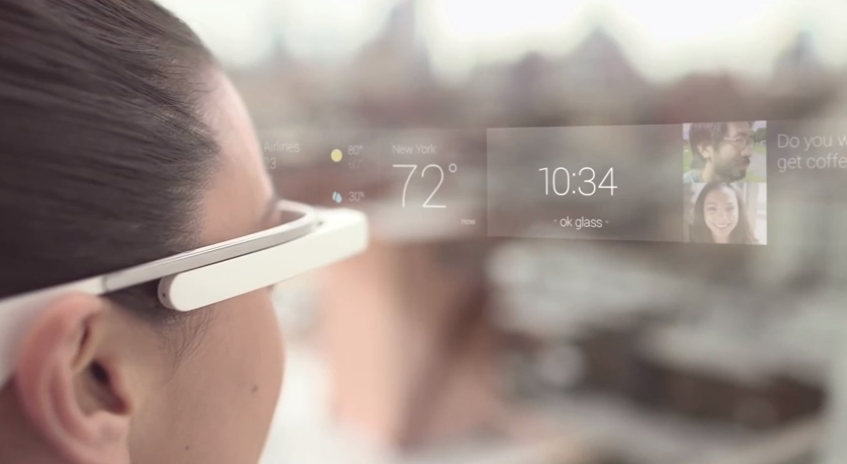
\includegraphics[width=110mm]{images/GoogleGlassUI}
		\caption{A visualisation of the timeline as the timeline is perceived by the user~\cite{ImagesGoogleGlassUI}.}
		\label{GoogleGlassUI}
	\end{figure}

The first screen the user sees when starting up Google Glass is the home screen. The home screen displays a clock and also shows the text "ok glass", as seen in Figure~\ref{GoogleGlassCards}~(a). The home screen is a part of the timeline and acts as the center point. Cards to the left of the home screen are upcoming activities such as an event in the user's calendar or an upcoming flight. Cards to the right of the home screen are from the past. Cards from the past will for instance show text messages or photos.

	\begin{figure}[ht!]
		\centering
   	\subfloat[The Google Glass home screen is a card that displays a clock.]{{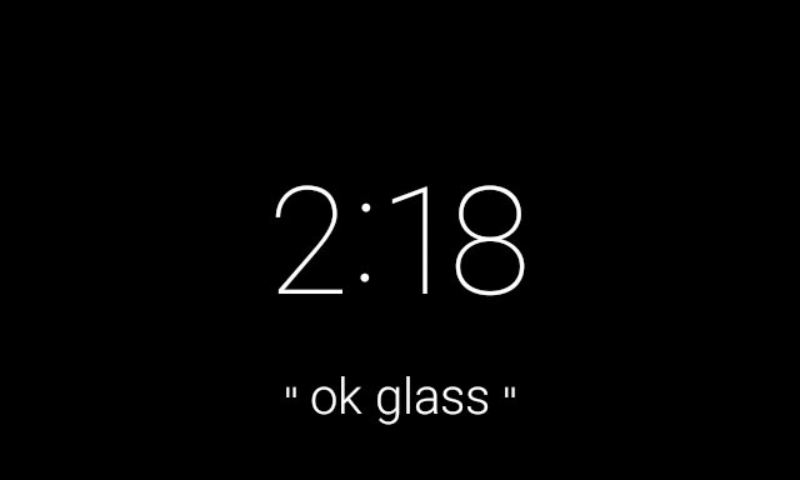
\includegraphics[width=70mm]{images/GoogleGlassHomescreen} }}
  	 \qquad
   	\subfloat[The card ``Explore stars'' represents an immersion.]{{
\includegraphics[width=70mm]{images/GoogleGlassStarImmersion} }}
   	\qquad
	\subfloat[The immersion ``Explore stars'' allows the user to look around at stars using the built-in head motion tracker.]{{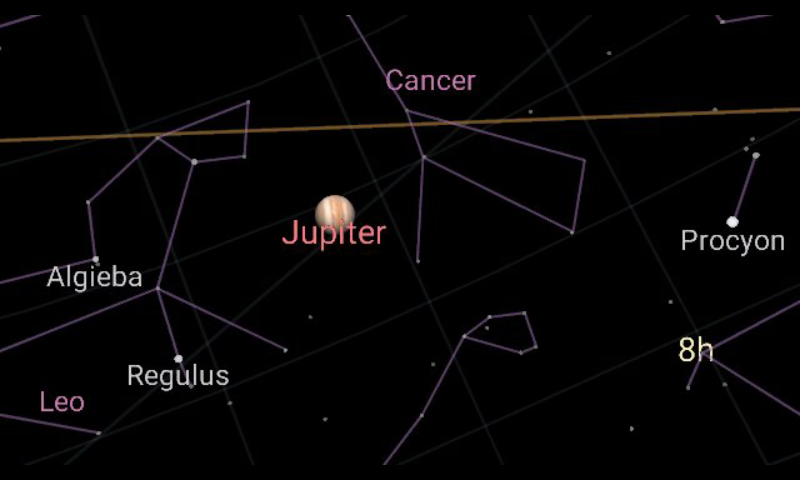
\includegraphics[width=70mm]{images/GoogleGlassStarImmersion2} }}
   	\qquad
		\caption{Cards can either display basic applications or represent immersions.}
		\label{GoogleGlassCards}
	\end{figure}

In order to move left on the timeline (forward in time) the user must swipe a finger backwards on the touchpad. In order to move right on the timeline (backward in time) the user must swipe a finger forward on the touchpad. The fact that the user must swipe backwards when stepping forward in time might not seem especially intuitive. In western culture a timeline is normally represented as going from left to right. One example is books, where the reader not only reads each line from left to right, but also turn pages from the right (the future) to the left (the past). However, on Google Glass, the swiping action could be thought of as swiping cards behind the back. Swiping forward when stepping backwards in time would then in turn mean bringing cards placed behind the back into focus. Cards in the past are behind the user while cards in the future are in front of the user.

When the user wants to turn off Google Glass the user swipes down on the touchpad. Swiping down on the touchpad will put Google Glass in stand-by mode. If the user wants to turn off Google Glass entirely, in other words power down the device, there is a power button on the opposite side of the touchpad. Holding down the power button for a few seconds will turn off Google Glass. For a better visual understanding of how Google Glass works see Figure~\ref{GoogleGlassUI} as well as the video referenced in the caption.

Google Glass uses a Bone Conduction Transducer (BCT) to transfer sound to the user~\cite{GlassSpecs}. The BCT transfers sound to the inner ear by conducting sound through the bones of the skull~\cite{boneConductionWiki}. The advantage of this technique is that the sound maintains clarity, even in noisy environments. Also, since the user does not plug any earphone into their ears, external sound is not blocked out.

Google Glass also features a 5 megapixels camera~\cite{GlassSpecs}. The camera sits between the touchpad and the display, as seen in Figure~\ref{GoogleGlassHardware}~(b), and is capable of capturing video at a 720p resolution. The camera can be used for video conferencing, as Google showed in 2012~\cite{glassLiveDemo}, but the camera can for instance also be used when the user wants to scan a QR Code (see Section~\ref{subsec:qrcode}).

The user can also interact with Google Glass using voice commands. As seen in Figure~\ref{GoogleGlassCards} the home screen consists not only of a clock but also of the words ``ok glass'', in quotes. ``ok glass'' indicates to the user that voice commands are available. The voice command menu is accessed as soon as the user says the words ``ok glass''. Doing so brings up a list of voice commands available, as seen in Figure~\ref{voiceCommandMenu}.

	\begin{figure}[H]%ht!]
		\centering
		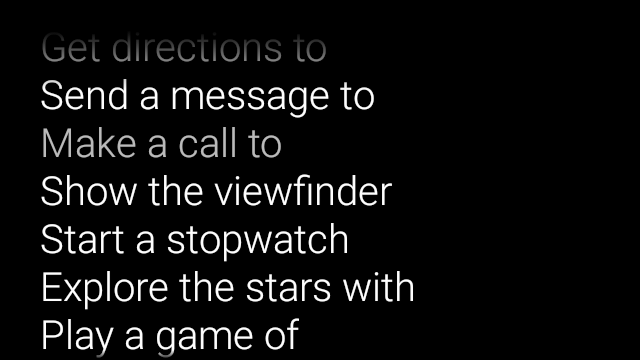
\includegraphics[width=110mm]{images/glassVoiceMenu}
		\caption{Saying ``ok glass'' will bring up the voice command menu~\cite{googleGlassVoiceCommand}.}
		\label{voiceCommandMenu}
	\end{figure}

In order to progress further the user must say one of the options being displayed out loud. Doing so will either make Google Glass perform the task spoken or give the user the option to add an input option to the task chosen. For instance, if the user where to say ``ok glass, Start a stopwatch'', Google Glass would start a stopwatch.

Google Glass also supports head motions as a form of input from the user. Head motions are not enabled in the timeline as a way of input but tilting the head may wake up Google Glass from stand by mode, if the user has enabled the head wake up feature~\cite{headWakeUp}. The head motion interface may also be used in certain immersions, such as ``Explore stars'' seen in Figure~\ref{GoogleGlassCards}~(c).
%The main way for a user to give input to Google Glass is via the touchpanel that is mounted on the right hand side of Glass, along the frame. Users are able to swipe as well as tap, which gives them control similar to that of a Smart TV's user interface. Where with a TV controller the user would maneuver with a simple cross layout (up, down, right and left) the buttons have on Glass been replaced by a touchpanel.\\

% Insert image of Google Glass graphical user interface here!!!

%The graphical interface is displayed at the top right through a projection coming from the right on a thick piece of glass. This technique lines up the image with the users sight but does not give any projection outwards.\\

%The interface is built with cards. Each card represents an activity.\\

%What’s unique?
%Standards?
%\url{https://developers.google.com/glass/design/}
%
\subsection{Compared to Smartphones}
\label{comparedtophones}
%Compare to phones!
Compared to smartphones one of the biggest advantages of Google Glass is the fact that Google Glass is a HMD. With a smartphone the user needs to either hold the smartphone in either one or both hands, alternatively put the smartphone on a table or the like. In other words can Google Glass offer a hands-free experience that smartphones can not.

Another advantage of Google Glass compared to smartphones is also comes from the fact that Google Glass is a HMD. The user does not need to look away in order to see what is currently being displayed. Google Glass does not distract from what the user is currently doing as much as a smartphone where the user needs to either look away or hold up the smartphone in from of the eyes.

However, smartphones does give the user a bit more control. The control comes from the fact that smartphones supports multi-touch, which Google Glass does not. On a smartphone users may also touch directly on the screen, in contrast to Google Glass where the touchpad sits on the right hand side of the user. Smartphones also have a larger touch area than Google Glass.

The smartphone screen size has been increasing ever since the iPhone first launched in 2007, as seen in Figure \ref{smartphoneSizeChart2}. Looking at currently available smartphones, in Figure \ref{smartphoneSizeChart}, the increase in screen size does not seem to stop as the average screen size is approaching five inches. In terms of comparison to Google Glass the increase in screen size entails that more information could be displayed on a smartphone than on Google Glass.

However, one of the biggest difference between smartphones and Google Glass is the plural. Smartphone\textbf{s}. There are several smartphone brands competing on the market, each offering several models. Google Glass is simply Google Glass, one products. As seen in section \ref{subsec:similarproducts} Google Glass does face competition that have approached HMDs differently, and as HMDs increase in popularity there is potential for an even wider offering of models and screen sizes.

%\url{https://developer.android.com/design/index.html}\\
%\url{https://developer.android.com/design/get-started/principles.html}
	\begin{figure}[ht!]
		\centering
		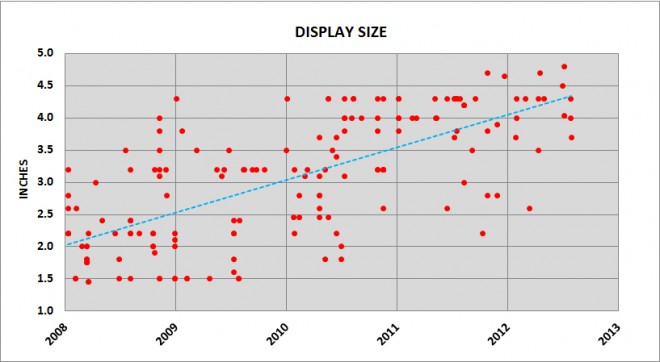
\includegraphics[width=110mm]{images/smartphoneSize2}
		\caption{Smartphone screens have been increasing ever since the iPhone launched in 2007.\cite{smartphoneSizeChart2}}
		\label{smartphoneSizeChart2}
	\end{figure}
	%http://www.pcworld.com/article/2455169/why-smartphone-screens-are-getting-bigger-specs-reveal-a-surprising-story.html

\hfill

%\url{https://developer.android.com/design/index.html}\\
%\url{https://developer.android.com/design/get-started/principles.html}
	\begin{figure}[ht!]
		\centering
		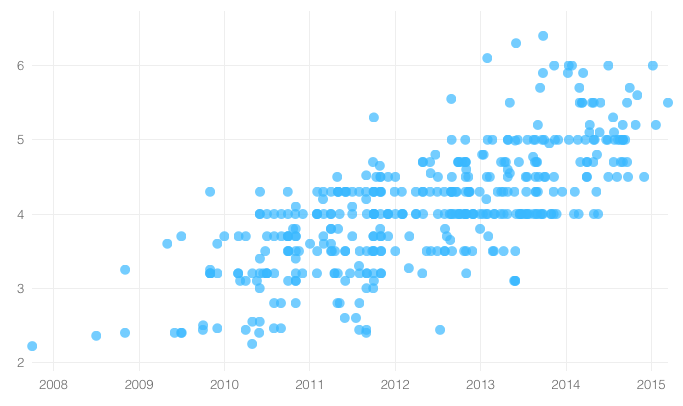
\includegraphics[width=110mm]{images/smartphoneSize}
		\caption{Smartphone screen sizes of the most popular of the currently available smartphones, where the x-axis shows the release date and the y-axis shows the screen size in inches.\cite{smartphoneSizeChart}}
		\label{smartphoneSizeChart}
	\end{figure}
	%http://www.pcworld.com/article/2455169/why-smartphone-screens-are-getting-bigger-specs-reveal-a-surprising-story.html

% Color schemes
% pre defined layouts
% pre defined typography (fonts)








%
\subsection{Limitations with Google Glass}
\label{subsec:limitations}
%Screen size
%Resolution
%Information on screen (possible result/discussion)
%How about people wearing glasses normally? Will the boss require employees to get lenses?
One early concern with Google Glass came from people who wore regular glasses every day, as Google Glass seemed to require separate frames. Isabelle Olsson at Google responded on the issue on April 12th 2012 with the following: ``We ideally want Project Glass to work for everyone, and we're experimenting with designs that are meant to be extendable to different types of frames.''~\cite{GoogleGlassFrameResponse}.

Today many eyecare providers have been trained for Google Glass and Glass frames. These trained eyecare providers are however mostly located in the United States~\cite{frameProviders}, but Google points out that many eyecare providers should be able to help replace the lenses on Google Glass' frames~\cite{framesGlass}.

% not relevant reference
%\url{http://www.google.com/glass/help/frames/} 
As described in an article posted on forbes in 2013~\cite{ackerman13}, a more alarming concern has been the health of the user's eyes. Concerns were raised regarding eye strain and misalignment of the user's eyes, as Google Glass placed a screen above one eye and not both. Google also saw these potential issues and approached Eli Peli, professor of ophthalmology who had been studying HMDs for two decades, as the development och Google Glass started.

Peli claimed that Google Glass has been designed with more safety and comfort in mind than previous, similar products. Peli pointed out that Google Glass is see-through and only covers a small part of the user's field of vision. As such Google Glass does not require a potentially poorly adjusted camera to capture the environment and display the environment to the user, which could cause eye strain.

Peli also pointed out that Google Glass is meant only to be used for short periods. Google Glass is meant to give the user notifications that can be quickly dealt with. The user should not be looking at the display for long periods of time, which would have the potential to lead to eye strain. While Peli stated that the risks are zero, he still claimed that the likelihood of Google Glass causing any damage is minimal.

%Eye pain? 
%\url{http://www.forbes.com/sites/eliseackerman/2013/03/04/could-google-glass-hurt-your-eyes-a-harvard-vision-scientist-and-project-glass-advisor-responds/}
%
%documented eye pain from looking at a screen for too long. Also conserns regarding looking at something that not both eyes can see. Can give headache and slighted eye aligntment.\\
%
Even though, according to Google's expert, there might not be any health risks involved, there is still a question of how much help Google Glass may be to users. A study performed in 2002~\cite{laramee02}, regarding the effects of OHMDs, showed that OHMDs may only be of help to users under controlled forms. Whenever the surrounding evnironment becomes too distracting, for instance within a moving crowd, performance decreases. The study however noted that pilots had been able to successfully turn HMD into a tool they could use to their advantage. Since the study was not carried out over a long period of time the participants were potentially not given enough time to get used to wearing and using their HMDs, explaining the poor performance when using a distracting background.

%HMD:s could potential be of great service to users as long as users take the time to get use to the HMD device.\cite{laramee02}\\
%
\subsection{QR Code}
\label{subsec:qrcode}
As mentioned in Section~\ref{subsec:userinterface}, Google Glass is equipped with a camera that could be used to take photos from the user's perspective. One potential use of the camera would be to scan QR codes. The QR Code was announced in 1994. Having been under development for several years at Denso Wave~\cite{qrCodeHistory}, the goal was to create a new form of barcode that could carry more information than a linear barcode and that could also be easily read.

A conventional barcode is capable of storing approximately 20 digits, while a QR code can store several thousand digits~\cite{qrCodeType}. In a QR code, information is encoded using standardised encoding modes and displayed as a 2D barcode. A QR code has several standardised fields, as seen in Figure~\ref{qrcodeMall}. Using position fields, a QR code can be read from any direction, compared to a conventional barcode which can only be read horizontally~\cite{qrCodeAbout}.

%	\begin{figure}[H]%ht!]
%		\centering
%		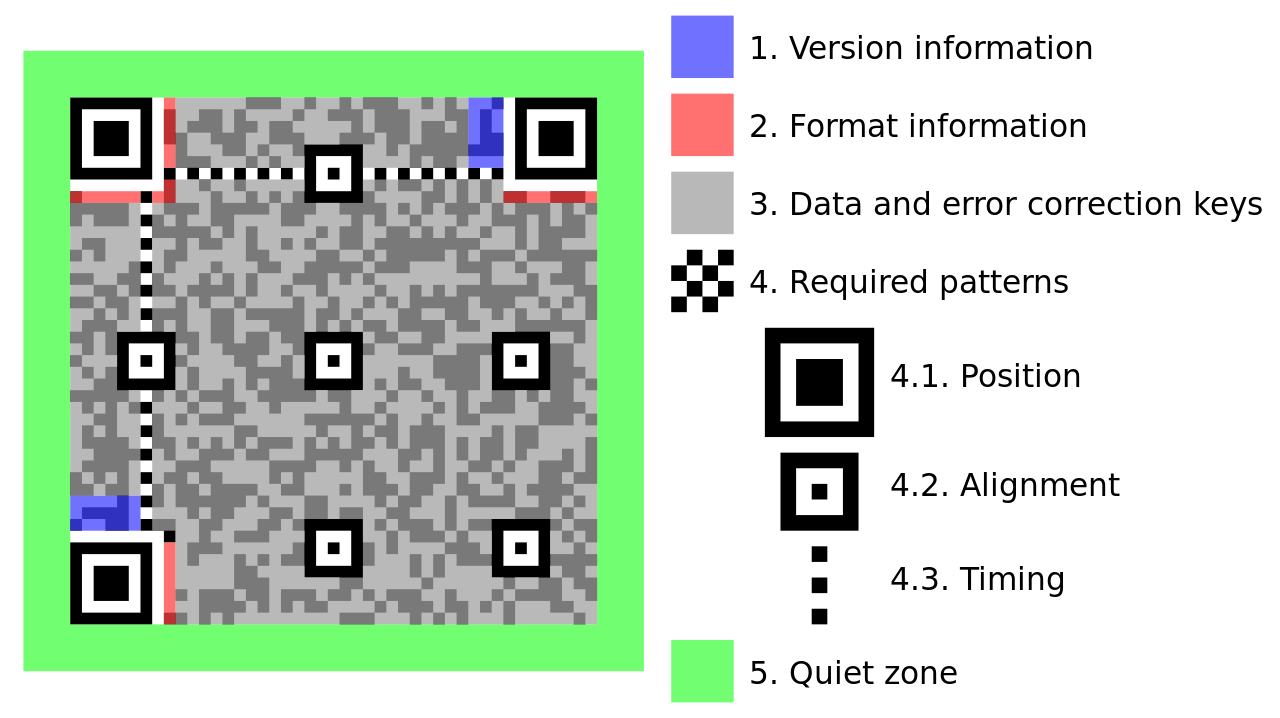
\includegraphics[width=110mm]{images/qrcodestandard}
%		\caption{The standardised fields in a QR Code~\cite{qrCodeWiki}.}
%		\label{qrcodestandard}
%	\end{figure}
	
	\begin{figure}[H]%ht!]
		\centering
		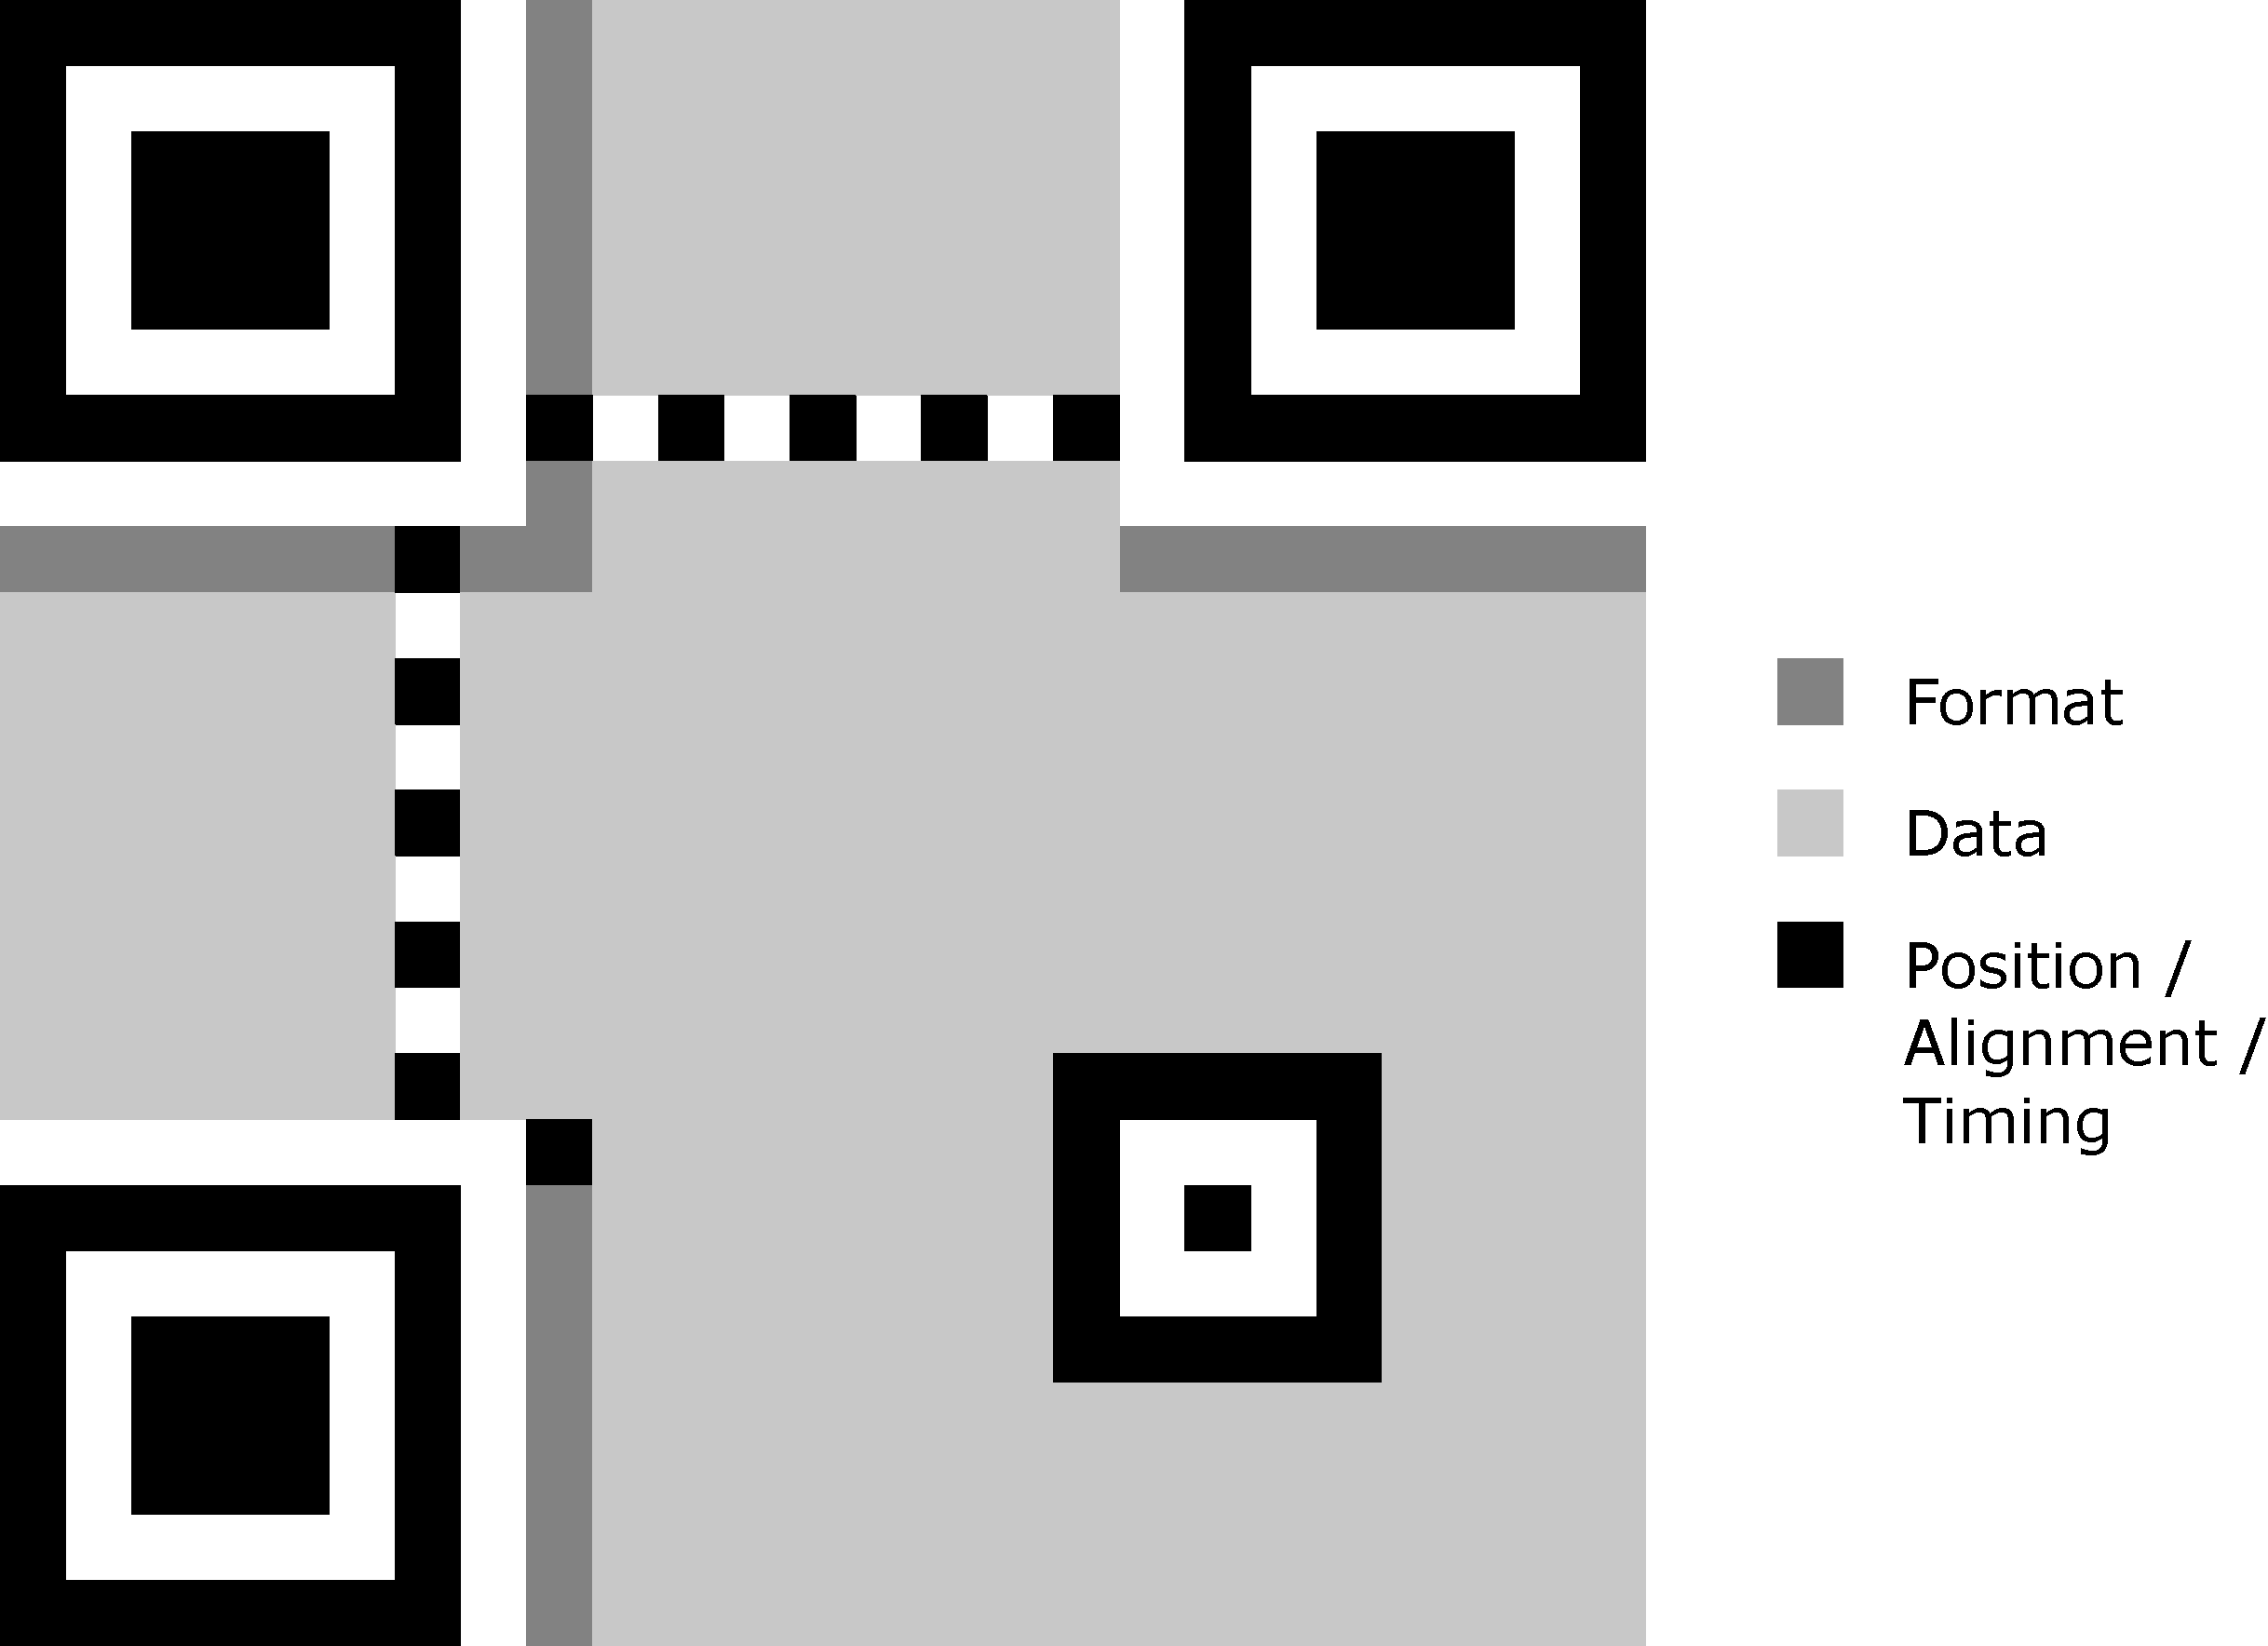
\includegraphics[width=80mm]{images/qrcodeMall}
		\caption{The standardised fields of a QR code~\cite{qrCodeWiki}.}
		\label{qrcodeMall}
	\end{figure}
	 
A QR code can be used to encode information, originally written with alphabetic characters, Japanese symbols (Kanji, Katakana and Hiragana) or numeric characters~\cite{qrCodeVersion}. With the help of a QR code, information which would otherwise have taken up a large space can now be easily fitted in smaller areas.

\subsubsection{Decoding}
Decoding a QR code is a fairly straight forward process which, although time consuming, can be done by hand, as described in several guides on the Internet~\cite{qrcodeDecoding2, qrcodeDecoding, qrcodeDecoding3}. A QR code may be divided in to three standardised fields, which help QR code scanners to identify and decode QR codes. The three fields can be seen in Figue~\ref{qrcodeMall}. The position, alignment and timing fields are used to identify and position the QR code correctly as a QR code may be scanned from any direction. In order to decode a QR code the three main position fields residing in three of the QR code's corners must be positioned as seen in Figure~\ref{qrcodeExample}.

The next step is to identify the mask used on the data field in the QR code. The mask is used to remove any large, empty or filled, areas within the data field which otherwise could make the decoding process more difficult for QR code scanners. The mask field is a part of the format field, seen in Figure~\ref{qrcodeMall}. The format field holds information about error correction, as well as which mask has been used on the data field. The mask is found among the first five bits in the format field. The first two bits of the first five bits of the format field contain information regarding the amount of error correction data the QR code contains, and the other three contain information on which mask has been used.

	\begin{figure}[H]%ht!]
		\centering
		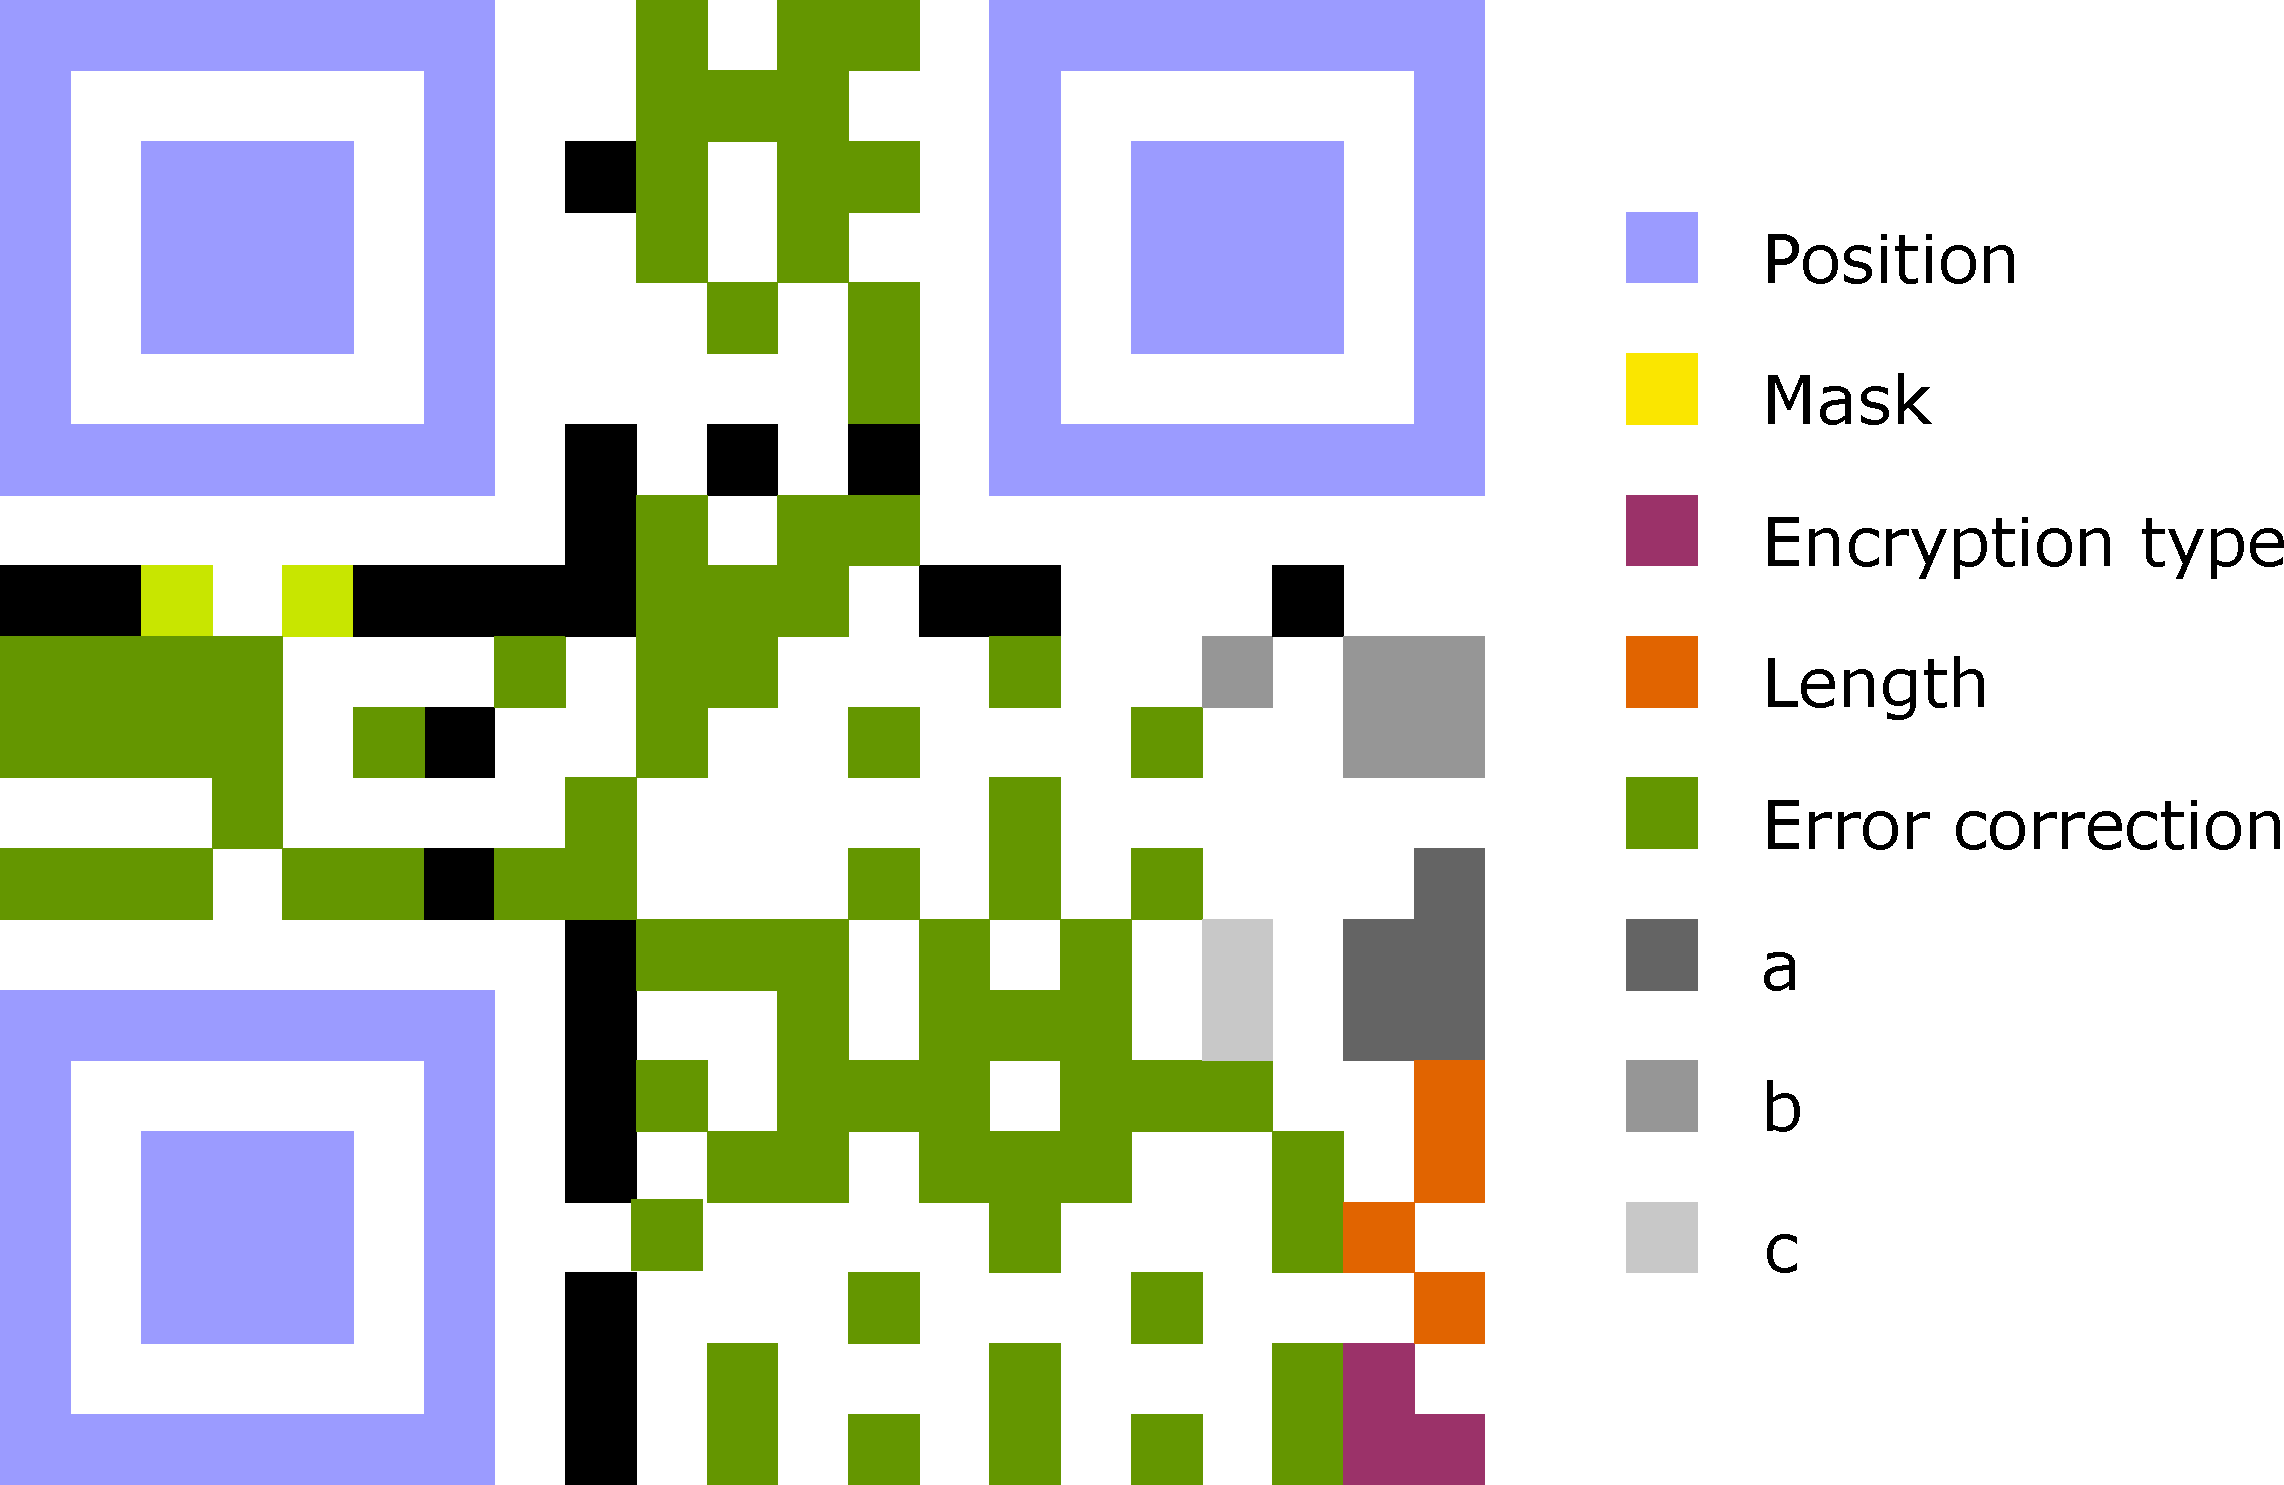
\includegraphics[width=100mm]{images/qrcodeexample}
		\caption{A QR code example, encoded with the string "abc".}
		\label{qrcodeExample}
	\end{figure}

In Figure~\ref{qrcodeExample} the mask field has the value of 101, seen more clearly in Figure~\ref{qrcodeExampleStep3}. Filled blocks should be interpreted as a 1 and empty blocks should be interpreted as a 0. However, the mask field is always XOR:d with 101 prior to being printed in the QR code and must as such be XOR:d back to the original mask value. In the case of Figure~\ref{qrcodeExample} the original mask value is calculated as follows:

\begin{center}
	101~XOR~101 = 000
\end{center}

	\begin{figure}[H]%ht!]
		\centering
		\fbox{
\includegraphics[width=30mm]{images/qrcodeexampleStep3}}
		\caption{Mask pattern encoded as 101.}
		\label{qrcodeExampleStep3}
	\end{figure}

There are eight different mask patterns in total, each represented by a unique bit string. The mask pattern represented by 000 can be seen in Figure~\ref{qrcodemaskpattern}, while the rest of the mask patterns may be found here~\cite{qrcodeMaskPatterns}. The mask used in Figure~\ref{qrcodeExample} means that a bit should be flipped when the following formula is true:

\begin{center}
	\((i+j)~mod~2=0\), 

	where i and j represent the indexes of the specific block, horizontally and vertically respectively~\cite{qrcodeMaskPatterns}.
\end{center}

	\begin{figure}[H]%ht!]
		\centering
		\fbox{
\includegraphics[width=40mm]{images/qrcodemaskpattern}}
		\caption{Mask pattern represented by the bit string 000~\cite{qrcodeMaskPatterns}.}
		\label{qrcodemaskpattern}
	\end{figure}
	
Having decoded the mask pattern the next step is to decode the data area. The data area always contains a header. The header contains information on the encryption type as well as data length. The blocks containing the encryption type are always the size of four blocks, and always located in the lower right corner, as seen in Figure~\ref{qrcodeExample}. The number of blocks used for the data length may vary between eight and ten blocks depending on the encryption type.

As such the first step in decoding the data area is to decode the encryption type. The information in the data area is to be read from the lower right and upwards, in a zig-zag pattern, with a width of two blocks. When reaching the top the zig-zag pattern continues, although downwards. See Figure~\ref{qrcodezigzag} for a better understanding of the zig-zag pattern. The start point is always in the lower right corner since the encryption type must be decoded first.

	\begin{figure}[H]%ht!]
		\centering
		
\includegraphics[width=100mm]{images/qrcodezigzag}
		\caption{The zig-zag pattern used when decoding a QR code.}
		\label{qrcodezigzag}
	\end{figure}

Using the zig-zag pattern, the encryption type bit string in Figure~\ref{qrcodeExample} can be found to be 1101, seen more clearly in Figure~\ref{qrcodeExampleStep4}. However, the encryption type is a part of the data section and as such must be unmasked. Using the mask formula gives the following results:

\begin{center}

\((20+20)~mod~2=40~mod~2=0\)

\((20+19)~mod~2=39~mod~2=1\)

\((19+20)~mod~2=39~mod~2=1\)

\((19+19)~mod~2=38~mod~2=0\)

\end{center}

	\begin{figure}[H]%ht!]
		\centering
		\fbox{
\includegraphics[width=15mm]{images/qrcodeexampleStep4}}
		\caption{Encryption type encoded as 1101.}
		\label{qrcodeExampleStep4}
	\end{figure}

As such the blocks at position (i, j) = (19, 19), and (i, j) = (20, 20) must be flipped. The ``flipping'' process may be done by XOR:ing the massked encryption type bit string with a bit string representing the bits that must be ``flipped'', putting ones at the positions where the corresponding bit in the masked encryption type bit string must be flipped, and zeroes at the position where the corresponding bit does not need to be flipped. The masked encryption type bit string, 1101, must as such be XOR:d with 1001, as follows:

\begin{center}
\(1101~XOR~1001=0100\)
\end{center}

There are several encryption types used in QR codes, however the most common ones are the following (represented by the following bit strings):

\begin{itemize}
	\item \itab{Numeric}		\tab{0001}
	\item \itab{Alphanumeric} 	\tab{0010}
	\item \itab{8-Bit Byte}		\tab{0100}
\end{itemize}

The encryption type used in Figure~\ref{qrcodeExample} is as such of encryption type 8-bit Byte.

After having decoded the encryption type the next step is to decode the length. The encoded length is the length of the message encoded in the QR code. Since the message encoded in the QR code may not cover the entire data section of the QR code (the rest is made up of error correction information) it is necessary to know the length of the message in order to tell when the message ends. Since the encryption type used in Figure~\ref{qrcodeExample} is an 8-bit Byte the size of each field that follows is eight bits in size.

The length field in Figure~\ref{qrcodeExample}, seen also in Figure~\ref{qrcodeExampleStep5}, is the following bit string: 10011010. However, the length field is a part of the data section and must as such be unmasked in order for the original length value to be obtained.

	\begin{figure}[H]%ht!]
		\centering
		\fbox{
\includegraphics[width=15mm]{images/qrcodeexampleStep5}}
		\caption{The message length encoded as 10011010.}
		\label{qrcodeExampleStep5}
	\end{figure}

\begin{center}

\((18+20)~mod~2=38~mod~2=0\)

\((18+19)~mod~2=37~mod~2=1\)

\((17+20)~mod~2=37~mod~2=1\)

\((17+19)~mod~2=36~mod~2=0\)

\((16+20)~mod~2=36~mod~2=0\) 

\((16+19)~mod~2=35~mod~2=1\)

\((15+20)~mod~2=35~mod~2=1\)

\((15+19)~mod~2=34~mod~2=0\)

\end{center}

The encryption type bit string must as such be XOR:d with 10011001, as follows:

\begin{center}
\(10011010~XOR~10011001=00000011=3\)
\end{center}

The message in Figure~\ref{qrcodeExample} is as such of length 3.

Finally, the data is decoded. The first 8-bit Byte, seen in Figure~\ref{qrcodeExampleStep6}, gives the following bit string: 11111000. However, being a part of the data section, the bit string must be unmasked, as follows:

\begin{center}

\((14+20)~mod~2=34~mod~2=0\)

\((14+19)~mod~2=33~mod~2=1\)

\((13+20)~mod~2=33~mod~2=1\)

\((13+19)~mod~2=32~mod~2=0\)

\((12+20)~mod~2=32~mod~2=0\) 

\((12+19)~mod~2=31~mod~2=1\)

\((11+20)~mod~2=31~mod~2=1\)

\((11+19)~mod~2=30~mod~2=0\)

\end{center}

The first 8-bit Byte bit string must as such be XOR:d with 10011001.

\begin{center}
\(11111000~XOR~10011001 = 01100001 = 64 + 32 + 1 = 97\)
\end{center}

	\begin{figure}[H]%ht!]
		\centering
		\fbox{
\includegraphics[width=15mm]{images/qrcodeexampleStep6}}
		\caption{The first 8-bit Byte encoded as 11111000.}
		\label{qrcodeExampleStep6}
	\end{figure}

The second 8-bit Byte, seen in Figure~\ref{qrcodeExampleStep7}, reaches the top of the data section and as such the last four bits must be read horizontally to the left, as described in Figure~\ref{qrcodezigzag}. Doing so gives the following bit string: 11110100. Again, the bit string must be unmasked.

\begin{center}

\((10+20)~mod~2=30~mod~2=0\)

\((10+19)~mod~2=29~mod~2=1\)

\((9+20)~mod~2=29~mod~2=1\)

\((9+19)~mod~2=28~mod~2=0\)

\((9+18)~mod~2=27~mod~2=1\) 

\((9+17)~mod~2=26~mod~2=0\)

\((10+18)~mod~2=28~mod~2=0\)

\((10+17)~mod~2=27~mod~2=1\)

\end{center}

The second 8-bit Byte bit string must as such be XOR:d with 10010110.

\begin{center}
\(11110100~XOR~10010110 = 01100010 = 64 + 32 + 2 = 98\)
\end{center}

	\begin{figure}[H]%ht!]
		\centering
		\fbox{
\includegraphics[width=30mm]{images/qrcodeexampleStep7}}
		\caption{The second 8-bit Byte encoded as 11110100.}
		\label{qrcodeExampleStep7}
	\end{figure}

The third, and final 8-bit Byte (seen in Figure~\ref{qrcodeExampleStep8}), to be decoded is read downwards, as described in Figure~\ref{qrcodezigzag}, giving the following bit string: 00000101. The bit string must be unmasked:

\begin{center}

\((11+18)~mod~2=29~mod~2=1\)

\((11+17)~mod~2=28~mod~2=0\)

\((12+18)~mod~2=30~mod~2=0\)

\((12+17)~mod~2=29~mod~2=1\)

\((13+18)~mod~2=31~mod~2=1\) 

\((13+17)~mod~2=30~mod~2=0\)

\((14+18)~mod~2=32~mod~2=0\)

\((14+17)~mod~2=31~mod~2=1\)

\end{center}

The third 8-bit Byte bit string must as such be XOR:d with 01100110.

\begin{center}
\(00000101~XOR~01100110 = 01100011 = 64 + 32 + 2 + 1 = 99\)
\end{center}

	\begin{figure}[H]%ht!]
		\centering
		\fbox{
\includegraphics[width=15mm]{images/qrcodeexampleStep8}}
		\caption{The third 8-bit Byte encoded as 00000101.}
		\label{qrcodeExampleStep8}
	\end{figure}

Since the message length was found to be of size 3, all parts of the message in Figure~\ref{qrcodeExample} have been found. The rest of the data section contains information regarding error correction, used in case the QR code was somehow damaged.

The message in Figure~\ref{qrcodeExample} has been decoded as 97, 98 and 99. Converting there numbers using an ASCII table gives the following result: a, b and c~\cite{asciitable}. The encoded message in Figure~\ref{qrcodeExample} has as such been decoded to ``abc'', which is correct and may be checked by scanning Figure~\ref{qrcodeExample} using a QR code scanner.

Although the decoding of a QR code may seem like an extensive process, the process may be divided in to the following five parts:

\begin{enumerate}
	\item Aligning the position
	\item Finding the mask used on the data section
	\item Unmasking the encryption type
	\item Unmasking the length of the encoded message
	\item Unmasking the message
\end{enumerate}

Although time consuming, decoding information from a QR code by hand is possible and follows the same steps as a QR code scanner.
%
\subsection{Information (and Ways of Presenting Information)}
\label{subsec:information}
In 1985 Sture All{\'e}n, professor of computational linguistics, and Einar Selander, honorary doctor at Ume{\aa} University, in their book---Information on Information---defined information after having gone through ``a large number of examples from texts of different kinds''.\cite{informationDef1} All{\'e}n and Selander defined information as ``a certain amount of facts or ideas''. While defining information can be done, there are several ways of presenting information.

\subsubsection{Text}
Text is one of the oldest forms of presenting information, with written text dating back to 4000 years B.C..\cite{cuneiform} Text is also a simple form of presentation that does not require much high end hardware. Other forms of presenting information require more memory, more computational power and more graphical power. Text also has the advantage that users can read through text at their own pace. Text does not have any perception of time.

Text does however have the disadvantage of requiring attention. The person reading the text must keep the attention on the text throughout and can not look away in order to receive all the information being presented. Text is also restricted to the language the text has been written in. In order to globalise a presentation of information in text several texts must be written so that users from different nations can read the text. For instance, English was in 2010 only the third most spoken language, behind Mandarin and Spanish.\cite{sprakNe} In other words would for instance this report require at least two translated versions in order to be globalised.

\subsubsection{Images}
The advantage of using images as the form of presenting information is that one can show the viewer the information rather than telling the viewer the information. Showing the viewer could potentially mean that more information could be presented within a smaller space than text could achieve. Images also gives the same advantage as text in terms of at what pace the viewer could perceive the information. Images, similar to text, does not have a perception of time.

Similar to text though, images require the viewers attention in order to present the information. The viewer can not look away from an image and still receive the information. Another disadvantage with images is the fact that images can be interpreted in different ways. The saying ``a picture is worth a thousand words'' goes both ways. On one hand images may present much information with one single image. On the other hand the information may not be crystal clear and not as clear cut as a describing text might be.

Images may also present information in two different way. One way is with photographs. Photographs may present abstract information and visualise what might be difficult to describe only using words. Another way of using images is by presenting information with graphs. Graphs are usually more clear cut in what information they want to present. However, graphs may in some cases be an insufficient way of presenting information. Graphs are used to present statistic information and are usually easier than photographs to translate into words. Statistic information, and as such also graphs, can summarise a period in time where as photographs captures a moment. 

\subsubsection{Audio}
Images and text both share the disadvantage of requiring full attention in order for the information to be perceived. Audio solves this problem. With audio as the form of presenting information the listener can look away and yet still receive the information that is being presented. In other words audio is well suited for multitasking as long as the other task the listener is performing does not involve listening to audio as well.

Audio does however have the disadvantage of not being insusceptible to time. The listener does not possess the same amount of control as he or she does with either text or images. Audio may be paused and rewinded but the fact that audio is still tied to a timeline is a disadvantage. Another disadvantage with audio is that, similar to text, audio is dependent on the language. If a information presentation were to be spread globally several audio files would be required (given that the audio contained spoken words) translated into different languages.

\subsubsection{Video}
Since video consist of many images bundled together video gives the same advantages as images in terms of showing the viewer the information instead of telling. Video presents the viewer with images at such speed that the images gives the impression of movement. Video may also include audio. The inclusion of audio potentially gives video all the same advantages as audio. In other words video could potentially give the advantages of two other forms of information presentation.

However, similar to audio, video is constantly moving. The viewer is bound to the playback speed of the video. Even though a video may be paused or even rewind the viewer does not possess the same amount of control as with images or text. With text and images the reader (or viewer) can deceide the pace at which the information should be perceived for themselves. If the video does not include audio video, similar to images or text requires full attention in order for the information to be perceived.
%
\subsection{Summary}
\label{subsec:summary}
%o   Introduce problem area / give relevant background info
%\\o   Introduction - Explain WHY you are doing this study
%\\o   Information - Background / your study in the wider context
%\\o   Similar work (projects, systems etc.)
%\\o   Summary - for this chapter
Google Glass was announced in 2012 along with the statement ``We think technology should work for you---to be there when you need it and get out of your way when you don't.''~\cite{GoogleGlassAnnouncement}. Google wanted to create a device where the user did not have to look down~\cite{tedtalkWhyGlass} as well as a device where the time between intention and action was minimised~\cite{6504855}. 

Google Glass (see Figure~\ref{GoogleGlassHardware}~(a) and~(b)) is an small HMD that is partially controlled with a touchpad mounted on the right hand side of the frames. The display sits slightly above the user's line of sight, on the right hand side. Google Glass' display is a projection that goes through an optic lense, creating a virtual image which makes the perception of the display to be equivalent of a 25 inch high definition screen seen from a distance of approximately 2.5 meters~\cite{GlassSpecs}.

Today there are many products similar to Google Glass either already on the market or in development. Microsoft Hololens is an HMD focused on letting the user work in a 3D space (with for instance 3D modelling~\cite{hololensDemo}) by covering both of the user's eyes. Recon Jet, GlassUp and C Wear Interactive Glasses are three products more similar to Google Glass in the sense that they only display information in front of one eye. However, Recon Jet is aimed at athletes, to be used while athletes are working out. GlassUp and C Wear Interactive Glasses are meant to be connected to an external device, such as a smartphone or a PC. Google Glass is a stand-alone device meant to be worn at all times.

The GUI of Google Glass is called a timeline and consists of a row of cards~\cite{ImagesGoogleGlassUI}. Cards are basic activities, such as a clock, but may also represent more in-depth applications, such as a game, on Google Glass called ``Immersions''. The center point of the timeline is the home screen and the first thing the user sees when turning on Google Glass. Cards to the left of the home screen are upcoming events, such as a flight, and cards to the right of the home screen are from the past, such as text messages. The user moves left on the timeline by swiping a finger backwards on the touchpad and in order to move right the user must swipe a finger forwards on the touchpad. 

In order to play sounds Google Glass uses a BCT which transfers sound through the bones of the skull~\cite{GlassSpecs}. The advantage of this technique is that external sound is not blocked out. In order to capture the environment Google Glass is also equipped with a 5 megapixles camera~\cite{GlassSpecs} and a microphone. Using the camera and the microphone the user may give input to Google Glass, for instance when using voice commands in order to control Google Glass hands-free.

The hands-free experience is also what sets Google Glass appart from regular smartphones. Smartphones must be held by the user or put on a table. The user must also look down at the screen of a smartphone, in contrast to Google Glass which puts the display slightly above the user's line of sight. Smartphones does however give the user a bit more control with multi-touch and touchscreen. Another advantage of smartphones is the larger screens. Smartphone screens have been increasing in size ever since the iPhone launched in 2007~\cite{smartphoneSizeChart2}. However, as HMDs increase in popularity, there is potential for a wider offering of models and screen sizes.

[TODO OVERGANG TILL QR KOD] The QR code was announced in 1994 by Denso Wave~\cite{qrCodeHistory}. The goal was to create a new form af barcode that could carry more information than a linear barcode and be easily read. While a conventional bardoce is capable of storing approximately 10 digits a QR code can store several thousand digits~\cite{qrCodeType}. A QR code also uses position fields which makes it readable from any direction, compared to a conventional barcode which can only be read horizontally~\cite{qrCodeAbout}. A QR code can be used to encode information, originally written with alphabetic characters, japanese symbols (Kanji) or numeric characters~\cite{qrCodeVersion}. 

information has been defined as ``a large number of examples from texts of different kinds''~\cite{informationDef1} and may be presented in a number of different ways. The four main ways of presenting information are text, images, sound and video. Text and images both have the advantage of being independent of time. Readers/viewers may perceive the information at their own pace. Images may also be divided into photographs and graphs. The difference of the two lies in the fact that graphs are used to present statistical information. Text and images does however both share the disadvantage of requiring readers/viewers vision.

Audio solves the problem of requiring the user's vision since audio uses a different sense. The listener may as a result multitask in terms of listening to the information being presented through audio while performing other tasks. For instance the listener may be listening to the radio while driving a car. In contrast to text and images audio is not independent of time.

Video shares the same disadvantage as audio in terms of not being independent of time. Video is, however, unique as video is the only form of presenting information which may combine images and show movement. Adding audio to video gives viewers the advantage of choice as they may choose to either watch or only listen.
[TODO SLUTKNORR PÅ KAPITLET]
%
%\subsection{Working handsfree}
%\label{subsec:workinghandsfree}
%Why?
%Multitasking (is this background or discussion?)
%Studies?
%\url{http://www.theguardian.com/science/2015/jan/18/modern-world-bad-for-brain-daniel-j-levitin-organized-mind-information-overload}
%\subsection{Multitasking on Google Glass}
%\label{subsec:multitaskingongoogleglass}
\cleardoublepage

\section{Design}
\label{sec:design}
%android studio vs eclipse with android sdk
%\url{http://wahidgazzah.olympe.in/integrating-zxing-in-your-android-app-as-standalone-scanner/}

%API level 12 because getIntent.getExtras.getString requires it. want default value there incase of error

o   Design - Present your project design in general
o   Information - Give details here (possibly several sub-sections)
\cleardoublepage

\section{Implementation}
\label{sec:implementation}
\subsection{Summary}
\label{subsec:summary}
The application works in such a way that the first screen the user sees when launching the application, on both Google Glass and smartphones, is the camera screen. The user is then to position the device in such a way that the QR code may be scanned by the device's camera. The QR code contains a product ID for a specific product.

The user does not need to press any shutter button in order to scan the QR code. Instead the application will automatically recognise any QR code pattern that appears in the camera view, as well as scan the QR code. The reason for not implementing a start menu or any similar start screen, to show the user before the camera screen is displayed, is to, according to Google's design guidelines, maintain the focus on what the application is intended to do and to keep the application simple and easy to use.

Next the application will decode the QR code. The decoding process is done by the ZXing library, which is an open source  barcode image processing library. The QR code contains a product ID which is then used in the downloading process. The downloading process entails connecting to a database containing information about different products, and, by using the decoded product ID, retrieving the information on the specific product. 

The downloaded information contains the product name, as well as a list of components and the instructions necessary to assemble the product. All the information is then sorted in to respective classes and the information may be displayed to the user. When the product information is being downloaded a loading animation is displayed on screen. On Google Glass the loading information is a loading bar at the bottom of the screen, and in the smartphone application the loading animation is a spinning wheel.

When the download process has finished the information is displayed to the user in the form of a slide show. The first slide that is displayed to the user is the title slide. The title slide contains the name of the product as well as an image  (if an image existed in the database). Following the title slide are the component slides. Each component has their own slide due to the fact that a component may be described in both text and an image. 

After all the component slides follow the instruction slides. Similar to the components an instruction my be presented by text only or by both text and an image. In contrast to the components, however, instructions may also be presented with an image and no text. 

As Google provides developers of Google Glass applications with predefined layouts, these layouts were also used for the Google Glass application. The layouts used were ``Title'', ``Columns'', ``Text'' and ``Caption''. The predefined layouts were also used as basis for the layouts used in the smartphone application.

The Title layout is used for the title card. The Columns layout is used for the slides with both text and an image. The Text layout is used for the slides with text only. The Caption layout is used for the slides containing only an image. All layouts, except for the Title layout, also contain text at the bottom of the screen called ``footer'' and ``timestamp''. The footer contains information on whether the current slide is a component slide or an instruction slide. The timestamp contains information on which slide is currently being viewed.

While browsing through the slides in the Google Glass application, the user may also navigate using voice commands. The voice commands available in the Google Glass application are ``Show next slide'', ``Show previous slide'', ``Show components'', ``Show instructions'' and ``Scan again''.

Most of the voice commands follow 11 out of the 15 voice command guidelines provided by Google. For example, ``Show components'' does not follow the guidelines which state that ``Is general enough to apply to multiple Glassware, but still has a clear purpose''. ``Show components'' is a specific voice command and could potentially apply to multiple Google Glass applications, but not all.

While viewing the slides ``ok glass'' is shown at the bottom of the screen. ``ok glass'' indicates that voice commands are available and saying ``ok glass'' at that point brings up the voice command menu, showing all available voice commands. However, ``ok glass'' is also shown in combination with a dark, transparent overlay, which ensures ``ok glass'' is always visible no matter what image is shown on screen, but the dark overlay also means that any image shown is darkened by the overlay.

In terms of the testing performed on the application, the experimental setup consisted of an optical bench on which the QR code was positioned at the zero mark, and then each specific device was positioned so that the camera of each device was positioned according to the specifications of each test. Each test result was then obtained through a laptop with which each device was connected via a USB cable. The test results were printed out from a timer class, called \texttt{Timer}, which was implemented using the singleton design pattern, meaning that the class had only one global instance which could be accessed from anywhere within the application.

The test which did not require the experimental setup was the text length test. Instead the text length test was performed using a class which randomised English characters, which were then concatenated together to form a longer string.

Three other tests were performed using the experimental setup. In the first of these three tests the distance to the QR code was varied. In the second test the complexity of the QR code was varied. In the third and final test the size of the downloaded information was varied. Each of these tests were performed 30 times, for each device and each different specification, to ensure statistical significance.

o   Implementation - Present your project implemetion in general
o   Information - Give details here (possibly several sub-sections)
o   Summary - for this chapter

% Mobile phone application
% Uses Zxing - library for QR code scanning [Link to gihub repository missing!!!]
% can display both text and images 
% 
% Google Glass Application
% Uses BarcodeEye - library for QR Code Scanning (port of Zxing for Google Glass) [Link to github repository missing!!!]
% Can display text, images still todo
% Much easier to add slides on Google Glass compared to Mobile Phone Application. Probably because Cards is standard interface for Google Glass (might also be because simple API, check CardPresenter!!!)
% Very difficult to add images since cards can't be changed after .getView() has been called
% Need to call .notifyViewChanged() but does not work anyway (yet) seems to only start the activity over which calls the execute method again if no check has been put in place
\cleardoublepage

\section{Results} % Result / Evaluation
\label{sec:resultevaluation}
The following are the results of the tests performed on the application, both on the Google Glass version as well as the smartphone version.

\subsection{Text Length}
The following are the results from evaluating the number of characters that may fit on a card in the Google Glass application, both when using only text and when using both text and an image. The test was performed only once for each device as despite randomising the characters used the text length would not differ significally from one case to another. As seen in the following results none of the tests resulted in an additional card with only one character. Had that been the case, different combinations of characters may have changed the number of cards necessary to display all of the information. As that is not the case only one test was deemed sufficient enough to determine the number of card required to display the same information as displayed on a smartphone device.

However, some trial and error was part of the process of finding how many characters would fill the smartphone screens. 550 was deemed a suitable number for Samsung Galaxy SII och 750 was deemed a suitable number for Samsung Galaxy SIII, as that many characters filled up the screen and yet still left some room for longer characters or longer words, as seen in Figure~\ref{glassTestTextLengthRaw}. For Samsung Galaxy SII, 600 characters did not fit on the screen, and for Samsung Galaxy SIII, 800 characters did not fit on the screen. As such 550 and 750 respectively was set as the maximum number of characters, although depending on the characters being displayed the text may use up more or less space as an 'i' does not take up as much space as a 'w'. The filled smartphone screens can be seen in Figure~\ref{glassTestTextLengthRaw}.

	\begin{figure}[H]%ht!]
		\centering
    		\subfloat[The Samsung Galaxy SII screen.]{{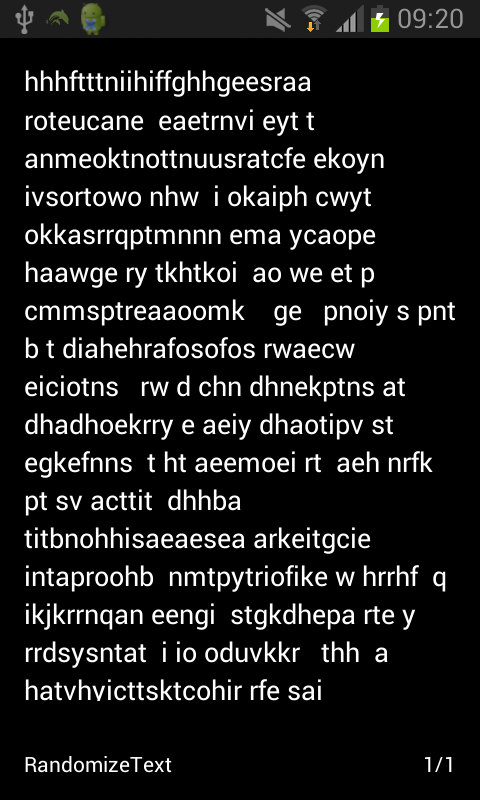
\includegraphics[width=50mm]{images/textLengthTestImages/S2_Raw}}}
   		 \qquad
		\subfloat[The Samsung Galaxy SIII screen.]{{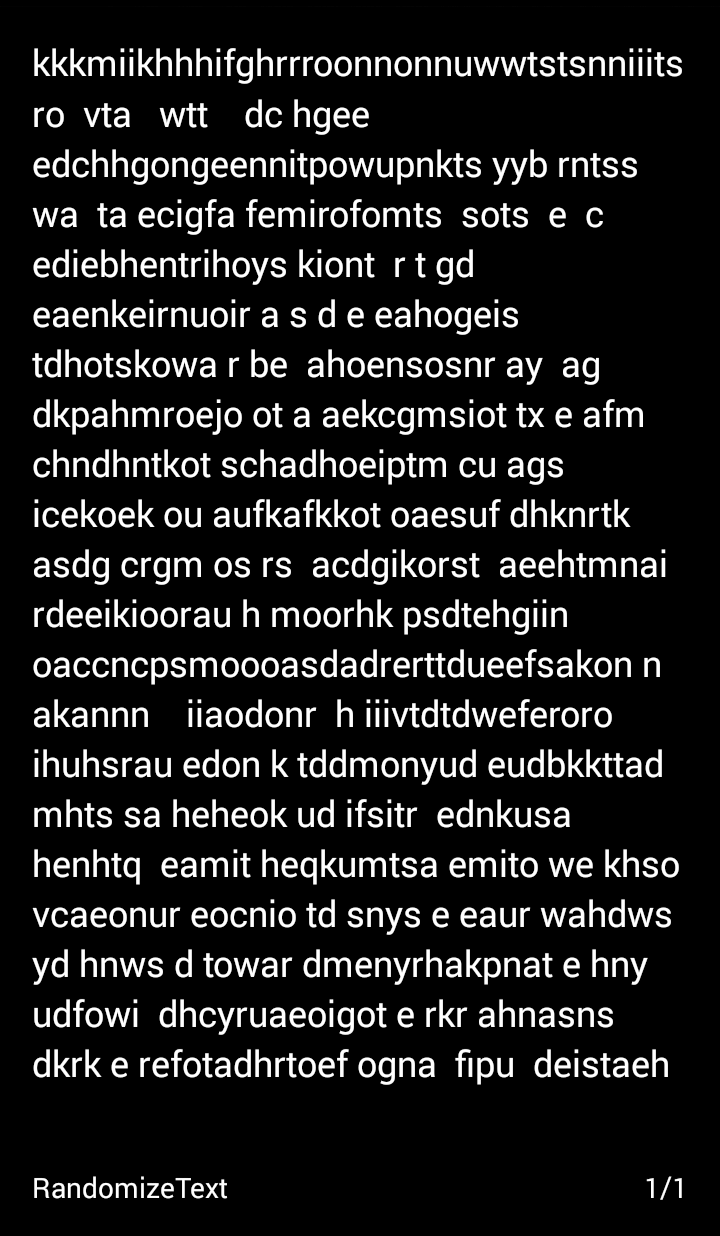
\includegraphics[width=50mm]{images/textLengthTestImages/S3_Raw}}}
   		 \qquad
		\caption{The maximum text length on the smartphone application.}
		\label{glassTestTextLengthRaw}
	\end{figure}

When translating the results from the smartphones to Google Glass the same text was used and simply copied over to the Google Glass application. The result of the text that filled the Samsug Galaxy SIII screen, seen in Figure~\ref{glassTestTextLengthRaw}~(a), can be seen in Figure~\ref{glassTestTextLengthS2Text}. As seen the text that filled the Samsung Galaxy SII screen took up roughly two and a half card in the Google Glass application. Although the screen is nearly filled in Figure~\ref{glassTestTextLengthS2Text}~(c) the text is dynamically sized depending on the amount of text being displayed. As such the card can be deemed about half full. Table~\ref{tab:glassTestTextLengthS2TextTable} shows the exact number of characters and words on each card, showing that the last card contains about half the number och characters as the other two cards.

	\begin{figure}[H]%ht!]
		\centering
    		\subfloat[The first slide.]{{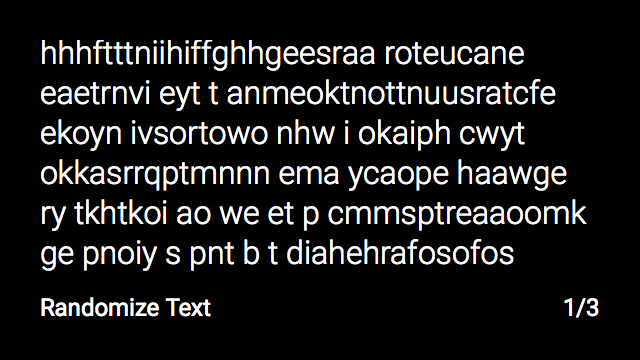
\includegraphics[width=60mm]{images/textLengthTestImages/S2_Text_1}}}
   		 \qquad
		\subfloat[The second slide.]{{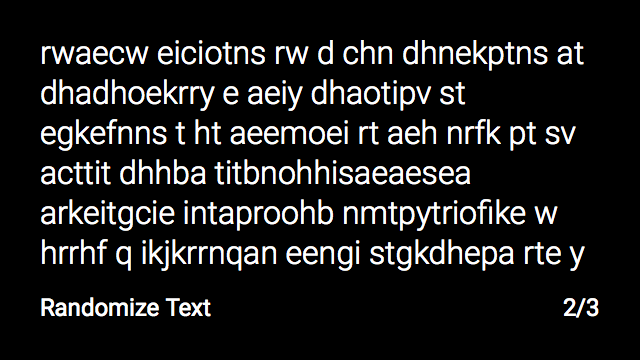
\includegraphics[width=60mm]{images/textLengthTestImages/S2_Text_2}}}
   		 \qquad
		\subfloat[The third slide.]{{
\includegraphics[width=60mm]{images/textLengthTestImages/S2_Text_3}}}
   		 \qquad
		\caption{Samsung Galaxy SII text.}
		\label{glassTestTextLengthS2Text}
	\end{figure}

	\begin{table}[ht!]
    		\caption{Details on text length on Google Glass from Samsung Galaxy SII.} \label{tab:glassTestTextLengthS2TextTable}
		\centering \begin{tabularx}{\textwidth}{l|X|X} \hline
		\textbf{Figure} & \textbf{Number of words} & \textbf{Number of characters} \\ \hline \hline
       
		Figure~\ref{glassTestTextLengthS2Text}~(a)	&30	&229	\\ \hline
		Figure~\ref{glassTestTextLengthS2Text}~(b)	&35	&229	\\ \hline
		Figure~\ref{glassTestTextLengthS2Text}~(c)	&13	&92	\\ \hline
		Figure~\ref{glassTestTextLengthS2Text}~(Total)	&78	&550	\\ \hline
		
		\end{tabularx}
	\end{table}

The result of using the text that filled the Samsung Galaxy SIII screen, seen in Figure~\ref{glassTestTextLengthRaw}~(b), in the Google Glass application can be seen in Figure~\ref{glassTestTextLengthS3Text}. As seen the Samsung Galaxy SIII screen fit more characters than the Samsung Galaxy SII screen and as such three and a half cards in the Google Glass application was needed to display all the text that filled the Samsung Galaxy SIII screen. The exact number och characters and words on each card can be seen in Table~\ref{tab:glassTestTextLengthS3TextTable}.

	\begin{figure}[H]%ht!]
		\centering
    		\subfloat[The first slide.]{{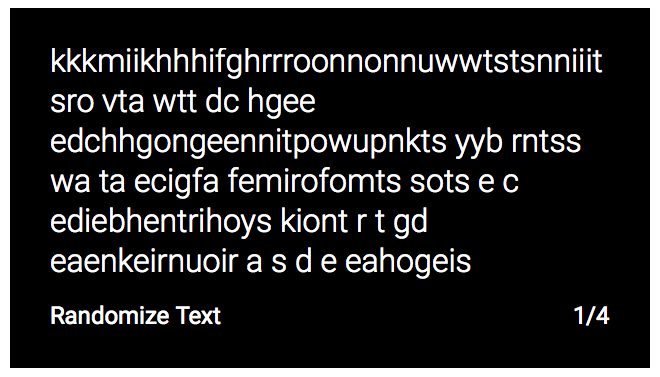
\includegraphics[width=60mm]{images/textLengthTestImages/S3_Text_1}}}
   		 \qquad
		\subfloat[The second slide.]{{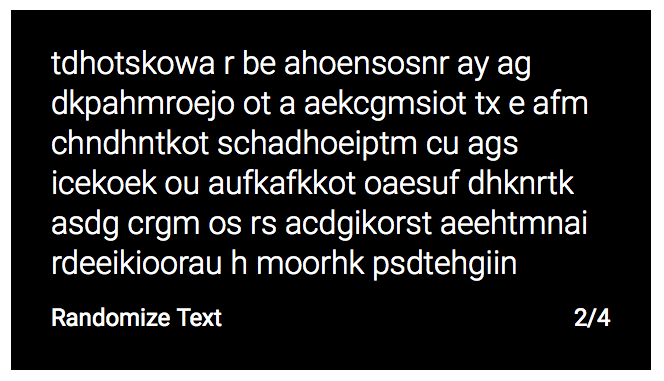
\includegraphics[width=60mm]{images/textLengthTestImages/S3_Text_2}}}
   		 \qquad
		\subfloat[The third slide.]{{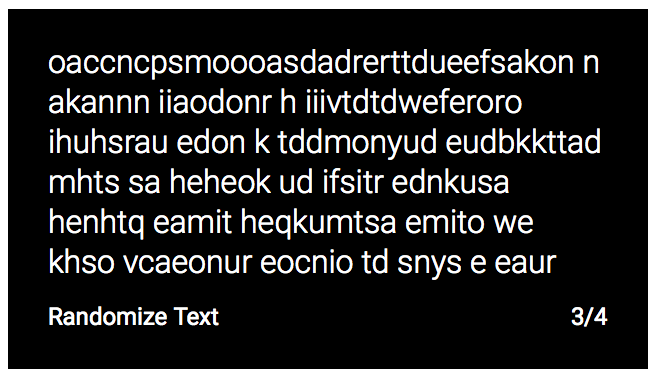
\includegraphics[width=60mm]{images/textLengthTestImages/S3_Text_3}}}
   		 \qquad
		\subfloat[The fourth slide.]{{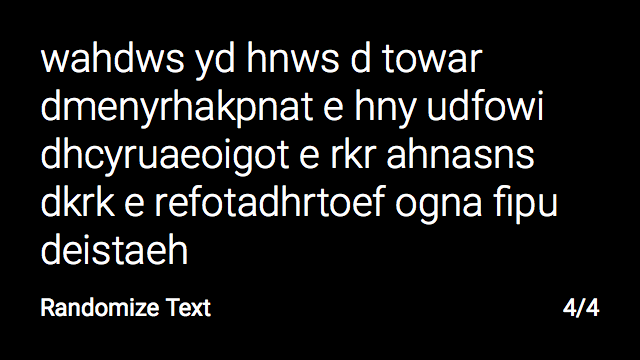
\includegraphics[width=60mm]{images/textLengthTestImages/S3_Text_4}}}
   		 \qquad
		\caption{Samsung Galaxy SIII text.}
		\label{glassTestTextLengthS3Text}
	\end{figure}

	\begin{table}[ht!]
    		\caption{Details on text length on Google Glass from Samsung Galaxy SIII.} \label{tab:glassTestTextLengthS3TextTable}
		\centering \begin{tabularx}{\textwidth}{l|X|X} \hline
		\textbf{Figure} & \textbf{Number of words} & \textbf{Number of characters} \\ \hline \hline
       
		Figure~\ref{glassTestTextLengthS3Text}~(a)	&26	&199	\\ \hline
		Figure~\ref{glassTestTextLengthS3Text}~(b)	&32	&213	\\ \hline
		Figure~\ref{glassTestTextLengthS3Text}~(c)	&29	&217	\\ \hline
		Figure~\ref{glassTestTextLengthS3Text}~(d)	&19	&121	\\ \hline
		Figure~\ref{glassTestTextLengthS3Text}~(Total)	&106	&750	\\ \hline
		
		\end{tabularx}
	\end{table}

Instructions described in text may also be displayed in combination with an image. When text combined with an image is used as the design layout for a slide the maximum number of characters that can be displayed changes. The image, according to Google's predefined card layout design~\cite{glassDesignStyle}, make up \(3/8\) of the card, and as such the text make up the other \(5/8\). As such the maximum number of characters can be calculated using the maximum number of characters used when presenting only text.

For Samsung Galaxy SII the maximum number of characters when using both text and an image was calculated as follows: \((5/8)*550~=~343.75\). As three quarters of a character is of no use the maximum number of characters on the Samsung Galaxy SII screen is 343 characters. The result of using the same text as when displaying only text on Samsung Galaxy SII, only shorten down to 343 characters can be seen in Figure~\ref{glassTestTextLengthS2Columns}, with specific numbers in Table~\ref{tab:glassTestTextLengthS2ColumnsTable}.

	\begin{figure}[H]%ht!]
		\centering
		\subfloat[The first slide.]{{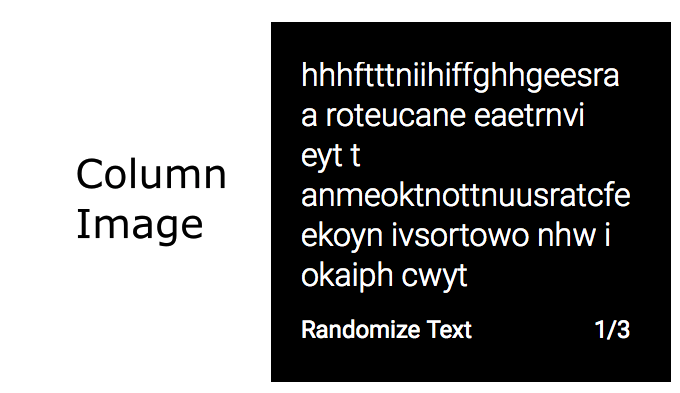
\includegraphics[width=60mm]{images/textLengthTestImages/S2_Columns_1}}}
   		 \qquad
		\subfloat[The second slide.]{{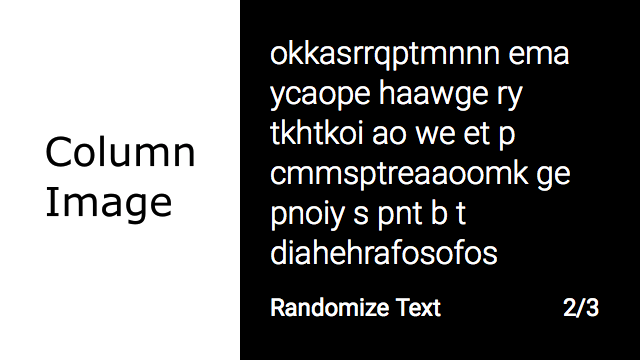
\includegraphics[width=60mm]{images/textLengthTestImages/S2_Columns_2}}}
   		 \qquad
		\subfloat[The third slide.]{{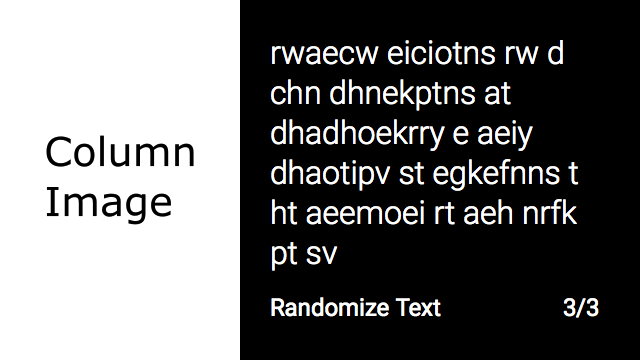
\includegraphics[width=60mm]{images/textLengthTestImages/S2_Columns_3}}}
   		 \qquad
		\caption{Samsung Galaxy SII text and image.}
		\label{glassTestTextLengthS2Columns}
	\end{figure}

	\begin{table}[ht!]
    		\caption{Details on text length on Google Glass from Samsung Galaxy SII.} \label{tab:glassTestTextLengthS2ColumnsTable}
		\centering \begin{tabularx}{\textwidth}{l|X|X} \hline
		\textbf{Figure} & \textbf{Number of words} & \textbf{Number of characters} \\ \hline \hline
       
		Figure~\ref{glassTestTextLengthS2Columns}~(a)	&12	&118	\\ \hline
		Figure~\ref{glassTestTextLengthS2Columns}~(b)	&18	&111	\\ \hline
		Figure~\ref{glassTestTextLengthS2Columns}~(c)	&21	&114	\\ \hline
		Figure~\ref{glassTestTextLengthS2Columns}~(Total)	&51	&343	\\ \hline
		
		\end{tabularx}
	\end{table}

The maximum number of characters when using both text and and image on Samsung Galaxy SIII was calculated the same way as for Samsung Galaxy SII, as follows: \((5/8~=~468.75)\). As three quarters of a character is of no use the maximum number of characters when displaying both text and an image is as such 468 characters. The result of using the same text as in Figure~\ref{glassTestTextLengthRaw}, only shorten down to 468 characters, in the Google Glass application can be seen in Figure~\ref{glassTestTextLengthS3Columns}. The application requires about three and a half card to be able to display all of the text. The exact number of characters and words on each card can be fount in Table~\ref{tab:glassTestTextLengthS3ColumnsTable}.

	\begin{figure}[H]%ht!]
		\centering
    		\subfloat[The first slide.]{{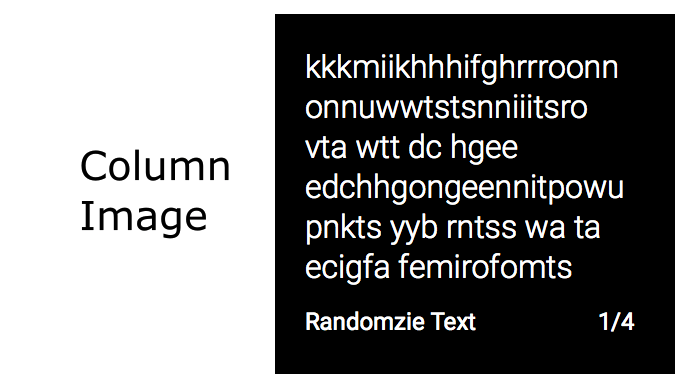
\includegraphics[width=60mm]{images/textLengthTestImages/S3_Columns_1}}}
   		 \qquad
		\subfloat[The second slide.]{{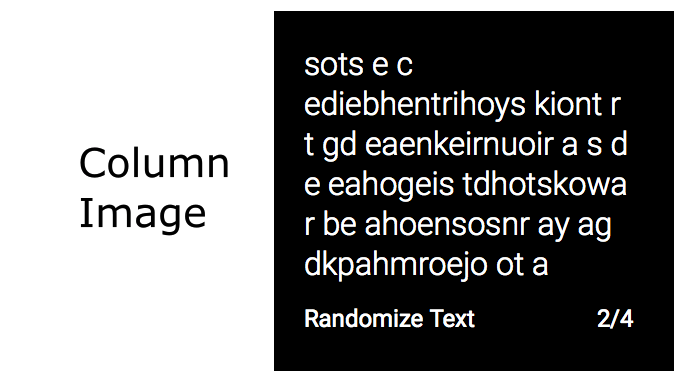
\includegraphics[width=60mm]{images/textLengthTestImages/S3_Columns_2}}}
   		 \qquad
		\subfloat[The third slide.]{{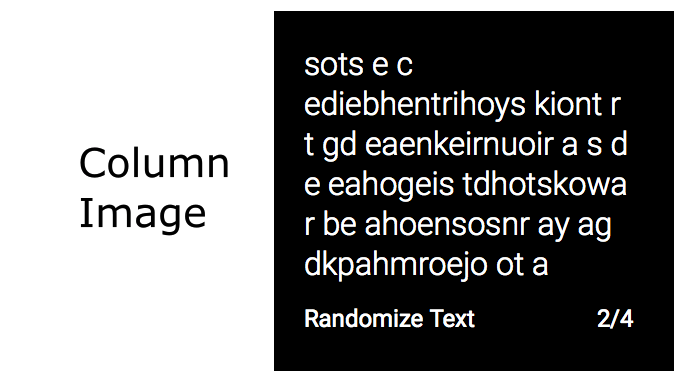
\includegraphics[width=60mm]{images/textLengthTestImages/S3_Columns_2}}}
   		 \qquad
		\subfloat[The fourth slide.]{{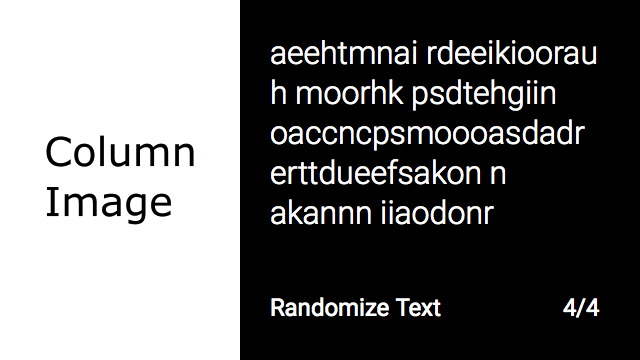
\includegraphics[width=60mm]{images/textLengthTestImages/S3_Columns_4}}}
   		 \qquad
		\caption{Samsung Galaxy SIII text and image.}
		\label{glassTestTextLengthS3Columns}
	\end{figure}

	\begin{table}[ht!]
    		\caption{Details on text length on Google Glass from Samsung Galaxy SIII.} \label{tab:glassTestTextLengthS3ColumnsTable}
		\centering \begin{tabularx}{\textwidth}{l|X|X} \hline
		\textbf{Figure} & \textbf{Number of words} & \textbf{Number of characters} \\ \hline \hline
       
		Figure~\ref{glassTestTextLengthS3Columns}~(a)	&12	&127	\\ \hline
		Figure~\ref{glassTestTextLengthS3Columns}~(b)	&23	&124	\\ \hline
		Figure~\ref{glassTestTextLengthS3Columns}~(c)	&18	&115	\\ \hline
		Figure~\ref{glassTestTextLengthS3Columns}~(d)	&9	&102	\\ \hline
		Figure~\ref{glassTestTextLengthS3Columns}~(Total)	&62	&468	\\ \hline
		
		\end{tabularx}
	\end{table}

Overall a slide in the Google Glass application, which contains only text, can fit around 200 characters, which corresponds to somewhere between 25 to 30 words. When using both text and and image the number of characters that may fit on a slide in the Google Glass application is about 115, which corresponds to about 15 words. In total the Google Glass application requires 3 to 4 cards for every slide in the smartphone application, depending on the size of the smartphone screen, in order to display the same text as a full slide in the smartphone application.

\subsection{Distance to the QR Code}

In Table~\ref{tab:distanceAverage} the average time for registering and decoding a QR code while varying the distance to the QR code can be seen. The size of the QR code was optimised for a distance of two decimeters between the QR code and the device, which also shows in the results as all devices registered the QR code fastest at a distance of two decimeters. The QR code used encoded only one character, an 'a'. The results from every individual run can be seen in Appendix~\ref{app:results}

	\begin{table}[H]%ht!]
    		\caption{Average time of registering a QR code with varying distance.} \label{tab:distanceAverage}
		\centering \begin{tabularx}{\textwidth}{l|X|X|X} \hline
		\textbf{Distance (dm)} & \textbf{Google Glass (sec)} & \textbf{Samsung Galaxy SII (sec)} & \textbf{Samsung Galaxy SIII (sec)} \\ \hline \hline
       
		1.0	&1.919976807	&1.965959850	&1.839656134	\\ \hline
		2.0	&1.831889852	&1.649790392	&1.487449920	\\ \hline
		3.0	&2.227158610	&1.921767210	&1.568837591	\\ \hline
		
		\end{tabularx}
	\end{table}

\subsection{Complexity of the QR Code}

Table~\ref{tab:complexityAverage} shows the average time for each device to both register and decode a QR code of varying complexity. The distance to the QR codes where two decimeters, as the size of the QR code was optimised for a distance of two decimeters between the QR code and the device. As seen in Table~\ref{tab:complexityAverage} some of the results are infinite, meaning that the device was never able to register the QR code due to the high complexity of the QR code. Samsung Galaxy SIII was able to both register and decode all three of the QR codes, Samsung Galaxy SII was not able to decode the most complex QR code and Google Glass was only able to register the simplest QR code.

One explanation as to why Google Glass was not able to register any QR code other than the simplest one would be that the Google Glass camera did not auto focus as well as both Samsung Galaxy SII and Samsung Galaxy SIII. As such the complexity of the QR code made it difficult to register the QR code. The difference can be seen in Figure~\ref{glassDemoQR}. Every single test run for each device can be found in Appendix~\ref{app:results}.

	\begin{table}[H]%ht!]
    		\caption{Average time of registering a QR code with varying density.} \label{tab:complexityAverage}
		\centering \begin{tabularx}{\textwidth}{l|X|X|X} \hline
		\textbf{Encoded Characters} & \textbf{Google Glass (sec)} & \textbf{Samsung Galaxy SII (sec)} & \textbf{Samsung Galaxy SIII (sec)} \\ \hline \hline
       
		1	&1.831889852	&1.649790392	&1.487449920	\\ \hline
		50	&\textit{Infinite}	&2.096434673	&1.913361687	\\ \hline
		100	&\textit{Infinite}	&\textit{Infinite}	&1.949743816	\\ \hline
		
		\end{tabularx}
	\end{table}

\subsection{Display Time}

The average display time of each device, with varying information sizes, can be seen in Table~\ref{tab:averageDisplaySpeedGoogleGlass}. As the size of the information increased, so did the average display time. The increase in time came as a result of all information being downloaded at the same time, and is then handled by the device. Although only the currently visible information is sent to the display, there are still more information handled by the device and as such the device must search through more information in order to determine what information is to be displayed. 

The display time is also affected by other background processes running at the same time. The average display time also only shows the time from when the information was sorted into classes until the information was sent to the display, and as such does not take in to account the potential delay the display might add in order to actually display the information to the user. Every single test run for each device can be found in Appendix~\ref{app:results}.

	\begin{table}[ht!]
    		\caption{Average display time for Google Glass with varying information size.} \label{tab:averageDisplaySpeedGoogleGlass}
		\centering \begin{tabularx}{\textwidth}{l|X|X|X} \hline
		\textbf{Information Size (Bytes)} & \textbf{Google Glass (sec)}  & \textbf{Samsung Galaxy SII (sec)}  & \textbf{Samsung Galaxy SIII (sec)} \\ \hline \hline
       
		1 000	&0.310802205	&0.008374156	&0.025498950	 \\ \hline
		100 000 	&0.442440796	&0.020444892	&0.034109654	 \\ \hline
		1 000 000	&0.582170613	&0.050938751	&0.078170083	 \\ \hline

		\end{tabularx}
	\end{table}


%%o   Introduction - Summarise your main results
%%o   Give details of the results
%%o   Best presentation? (text, tables, diagrams?)
%o   Implementation Evaluation - your results against your expectations%
%%o   Summary - for this chapter

%\subsection{The Application}

%\subsubsection{Google Glass}

%\subsubsection{Smartphone}

%\subsection{Test Cases}

%\subsubsection{Text Length}

%\subsubsection{Image Size}

%\subsubsection{Comparing Text and Images}

%\subsubsection{Download Speed}

%\subsubsection{Interaction Delay}

%\subsubsection{Background Noise}

%\subsubsection{Size of QR Code}

%\subsubsection{Complexity of QR Code}

%\subsubsection{``Tap Counter''}

%\subsubsection{User Experience}

%\subsubsection{Multitasking}

%\subsubsection{Battery}

%\subsubsection{Connected to Mobile Device}

%\subsubsection{Overall Conclusions}
\cleardoublepage

\section{Conclusions}
\label{sec:conclusion}
o   Conclusion
o   Project Evaluation
o   Problems - How would you do this the next time?
o   Future work
\cleardoublepage

%\nocite{*}

% Start of reference section. 
\begin{singlespace}
\bibliography{myBibliography}
\bibliographystyle{plain}
\end{singlespace}
\cleardoublepage

% Appendix if present goes here (optional part)
\appendix
\section{Abbreviations}
\label{sec:abbreviations}
\begin{description}
	\item [2D] Two-Dimensional
	\item [3D] Three-Dimensional
	\item [API] Application Programming Interface
	\item [BCT] Bone Conduction Transducer
	\item [GDK] Glass Development Kit
	\item [GUI] Graphical User Interface
	\item [HMD] Head-Mounted Display
	\item [HUD] Heads-Up Display
	\item [IDE] Integrated Development Environment
	\item [OHMD] Optical Head-Mounted Display
	\item [QR Code] Quick Response Code
	\item [ZXing] Zebra Crossing
\end{description}
\cleardoublepage

\section{Results}
\label{app:results}
	\begin{table}[ht!]
    		\caption{Google Glass} \label{tab:distamceSmartphoneFull}
		\centering \begin{tabularx}{\textwidth}{l|X|X|X} \hline
		\textbf{Test Number} & \textbf{1 decimeter} & \textbf{2 decimeters} & \textbf{3 decimeters} \\ \hline \hline
       
		1&	1884216308	&	1798065186	&	2296325683	\\ \hline
		2&	1682800293	&	1705902100	&	2415893555	\\ \hline
		3&	2043151856	&	1937561035	&	2408782959	\\ \hline
		4&	2487091065	&	1779327392	&	2346679688	\\ \hline
		5&	1316070557	&	1948822022	&	2336975098	\\ \hline
		6&	1631652832	&	1777801514	&	2341278076	\\ \hline
		7&	1576843262	&	1941070556	&	2184875488	\\ \hline
		8&	1772125244	&	2041961670	&	2347503662	\\ \hline
		9&	2140167236	&	2060516358	&	2296203613	\\ \hline
		10&	1911987304	&	1757171630	&	2170745849	\\ \hline
		11&	1884277345	&	1767211914	&	2357238769	\\ \hline
		12&	1929656983	&	2313415528	&	2337341308	\\ \hline
		13&	1709838868	&	1731719971	&	2460479736	\\ \hline
		14&	1819946288	&	1789154053	&	2208862304	\\ \hline
		15&	1881225586	&	1959869384	&	2198150634	\\ \hline
		16&	1790405272	&	1852996826	&	2317962646	\\ \hline
		17&	1574829101	&	1649383545	&	1774505615	\\ \hline
		18&	1825531006	&	1702728271	&	2231719971	\\ \hline
		19&	1731201172	&	1674377441	&	2281311035	\\ \hline
		20&	2475097657	&	1735839844	&	1698455811	\\ \hline
		21&	2370330810	&	1776123047	&	2375762940	\\ \hline
		22&	1872375489	&	1714141846	&	2186004639	\\ \hline
		23&	2327819824	&	2099090575	&	2258178712	\\ \hline
		24&	1753479003	&	1826843263	&	2193664551	\\ \hline
		25&	1721496582	&	1849182128	&	2280761718	\\ \hline
		26&	2481842039	&	1802490234	&	1814788818	\\ \hline
		27&	1602935791	&	1912353515	&	1650085449	\\ \hline
		28&	2181121826	&	1636383056	&	2349945068	\\ \hline
		29&	1797210694	&	1716491699	&	2250000000	\\ \hline
		30&	2422576904	&	1698699951	&	2444274902	\\ \hline

		\end{tabularx}
	\end{table}

	\begin{table}[ht!]
    		\caption{Samsung Galaxy SII} \label{tab:distamceGoogleGlassFull}
		\centering \begin{tabularx}{\textwidth}{l|X|X|X} \hline
		Test Number & \textbf{1 decimeter} & \textbf{2 decimeters} & \textbf{3 decimeters} \\ \hline \hline
		
		1&	2139868085	&	1486211750	&	1643240375	\\ \hline
		2&	1467511210	&	1433458333	&	1645772458	\\ \hline
		3&	1531975085	&	1544185626	&	2269734332	\\ \hline
		4&	1999989252	&	1474127458	&	1652179501	\\ \hline
		5&	2117759919	&	1437559418	&	1784042751	\\ \hline
		6&	1590932000	&	1346899542	&	1959105167	\\ \hline
		7&	2309159125	&	1542022917	&	2183700002	\\ \hline
		8&	1722160542	&	1421151250	&	1430372917	\\ \hline
		9&	1442118042	&	1537669377	&	2517021085	\\ \hline
		10&	2225043835	&	1922686667	&	1584863210	\\ \hline
		11&	2559335792	&	1634340084	&	1544045376	\\ \hline
		12&	2087568125	&	1493966751	&	2455554542	\\ \hline
		13&	2399355752	&	1654488126	&	2096796210	\\ \hline
		14&	1835165960	&	1681548458	&	1444782750	\\ \hline
		15&	2013470417	&	1577887875	&	2794100627	\\ \hline
		16&	1947420919	&	1971720543	&	2164583833	\\ \hline
		17&	1914936335	&	1497237917	&	1976264377	\\ \hline
		18&	1964812292	&	1473154916	&	2001674627	\\ \hline
		19&	1836791835	&	1332783794	&	2090852043	\\ \hline
		20&	1291630877	&	1760558543	&	1331759376	\\ \hline
		21&	1715746333	&	1808396667	&	1840536334	\\ \hline
		22&	2281021168	&	1940200418	&	2039864458	\\ \hline
		23&	2106378627	&	1551906084	&	2214860250	\\ \hline
		24&	2048848293	&	2127196127	&	1541294919	\\ \hline
		25&	1953401960	&	1389226667	&	1873071125	\\ \hline
		26&	1901472292	&	1534745500	&	2040191418	\\ \hline
		27&	2009275501	&	1439262916	&	1916855625	\\ \hline
		28&	1843962793	&	2145346709	&	1627921959	\\ \hline
		29&	2639261585	&	2315900375	&	1939550709	\\ \hline
		30&	2082421543	&	2017870959	&	2048423918	\\ \hline
		
		\end{tabularx}
	\end{table}
	
	\begin{table}[ht!]
    		\caption{Samsung Galaxy SIII} \label{tab:distamceGoogleGlassFull}
		\centering \begin{tabularx}{\textwidth}{l|X|X|X} \hline
		Test Number & \textbf{1 decimeter} & \textbf{2 decimeters} & \textbf{3 decimeters} \\ \hline \hline
		
		1&	1749676834	&	1779497917	&	1513588627	\\ \hline
		2&	1980956916	&	1389859375	&	1552651834	\\ \hline
		3&	1784749169	&	1264649875	&	1513143459	\\ \hline
		4&	1842951960	&	1513206585	&	1352977542	\\ \hline
		5&	1754621419	&	1473651001	&	1307146084	\\ \hline
		6&	1644033335	&	1392401627	&	1453716167	\\ \hline
		7&	1730130585	&	1282980458	&	1582548250	\\ \hline
		8&	1672027044	&	1688112459	&	1311798583	\\ \hline
		9&	1737328751	&	1432261543	&	1462818377	\\ \hline
		10&	2373175125	&	1317017667	&	1316425376	\\ \hline
		11&	1848027542	&	1463129292	&	2047718001	\\ \hline
		12&	1576518375	&	1676956292	&	1675308210	\\ \hline
		13&	1642278708	&	1709122334	&	1916630376	\\ \hline
		14&	1750943335	&	1423191250	&	2168636127	\\ \hline
		15&	1792001168	&	1402313542	&	1774322918	\\ \hline
		16&	1733112083	&	1544061083	&	1798746335	\\ \hline
		17&	2075140127	&	1554050960	&	2053470334	\\ \hline
		18&	1940637085	&	1406057500	&	1583177875	\\ \hline
		19&	1879888500	&	1666031252	&	1327241125	\\ \hline
		20&	1690253250	&	1350420626	&	1350043708	\\ \hline
		21&	1694755291	&	1506406918	&	1429665709	\\ \hline
		22&	1966512835	&	1445166958	&	1401702668	\\ \hline
		23&	1741643376	&	1664807709	&	1242497667	\\ \hline
		24&	2036178543	&	1692449501	&	1511735834	\\ \hline
		25&	1694977000	&	1474073667	&	1383570126	\\ \hline
		26&	1851916252	&	1655224458	&	1549562168	\\ \hline
		27&	1653187293	&	1203773709	&	1560395085	\\ \hline
		28&	1966861500	&	1297300542	&	1317753292	\\ \hline
		29&	1885895208	&	1287375710	&	1785062417	\\ \hline
		30&	2499305419	&	1667945793	&	1821073459	\\ \hline

		\end{tabularx}
	\end{table}
\input{tables/ComplexityTable.tex}
	\begin{table}[ht!]
    		\caption{Google Glass} \label{tab:distamceSmartphoneFull}
		\centering \begin{tabularx}{\textwidth}{l|X|X|X} \hline
		Test Number & \textbf{1 kB} & \textbf{100 kB} & \textbf{1 MB} \\ \hline \hline

		1&	22128417	&	23806542	&	21965000	\\ \hline
		2&	15872960	&	25955458	&	23531209	\\ \hline
		3&	22888792	&	35965208	&	19634833	\\ \hline
		4&	28067583	&	38730916	&	24453667	\\ \hline
		5&	19896250	&	38804333	&	32512083	\\ \hline
		6&	23419042	&	29999625	&	26414750	\\ \hline
		7&	21411542	&	38175167	&	24274417	\\ \hline
		8&	26785041	&	31706084	&	27390000	\\ \hline
		9&	22456042	&	36254834	&	24890666	\\ \hline
		10&	21889541	&	35148375	&	28355083	\\ \hline
		11&	27834042	&	42737374	&	23042333	\\ \hline
		12&	22855541	&	42614042	&	25686667	\\ \hline
		13&	26527083	&	28933625	&	27155416	\\ \hline
		14&	23235959	&	22850875	&	26465708	\\ \hline
		15&	21809916	&	38291375	&	25557583	\\ \hline
		16&	20713958	&	24469625	&	25121875	\\ \hline
		17&	21938833	&	32561208	&	22315125	\\ \hline
		18&	22112709	&	48090375	&	20184625	\\ \hline
		19&	26409875	&	30071209	&	20032209	\\ \hline
		20&	27796334	&	27028876	&	19081542	\\ \hline
		21&	22990750	&	31401792	&	27814292	\\ \hline
		22&	22468667	&	31754459	&	17277167	\\ \hline
		23&	15608750	&	31208458	&	24796125	\\ \hline
		24&	22743958	&	30416209	&	25758250	\\ \hline
		25&	25656166	&	22642625	&	18390541	\\ \hline
		26&	21030250	&	22831791	&	18389583	\\ \hline
		27&	25625666	&	25375541	&	20224416	\\ \hline
		28&	21925167	&	48635958	&	18421000	\\ \hline
		29&	22280792	&	23115125	&	20458334	\\ \hline
		30&	22374167	&	42448750	&	18195875	\\ \hline
		
		\end{tabularx}
	\end{table}

	\begin{table}[ht!]
    		\caption{Samsung Galaxy SII} \label{tab:distamceGoogleGlassFull}
		\centering \begin{tabularx}{\textwidth}{l|X|X|X} \hline
		Test Number & \textbf{1 kB} & \textbf{100 kB} & \textbf{1 MB} \\ \hline \hline
       
		1&	6797250	&	14496709	&	64364083		\\ \hline
		2&	6326709	&	43183958	&	100282458	\\ \hline
		3&	6746292	&	24071374	&	18386459		\\ \hline
		4&	7058875	&	31881374	&	80973374		\\ \hline
		5&	11829542	&	28462958	&	84470625		\\ \hline
		6&	10667375	&	13489125	&	109992750	\\ \hline
		7&	8890167	&	12720376	&	18701084		\\ \hline
		8&	21200959	&	28104084	&	11930708		\\ \hline
		9&	5742833	&	14041624	&	37545749		\\ \hline
		10&	7117500	&	34152708	&	37839583		\\ \hline
		11&	6092042	&	13555542	&	32261416		\\ \hline
		12&	7110333	&	14802667	&	26862500		\\ \hline
		13&	11012625	&	14330666	&	32655250		\\ \hline
		14&	9552500	&	29462791	&	38692001		\\ \hline
		15&	8780000	&	40578625	&	73218541		\\ \hline
		16&	10533500	&	11147917	&	11013791		\\ \hline
		17&	5902250	&	13767874	&	10906625		\\ \hline
		18&	10135791	&	12711084	&	137211250	\\ \hline
		19&	8074709	&	13150458	&	29192460		\\ \hline
		20&	8935250	&	13934084	&	102380958	\\ \hline
		21&	6071583	&	14262083	&	29384416		\\ \hline
		22&	6577125	&	15152625	&	31167750		\\ \hline
		23&	6078875	&	23965041	&	32326793		\\ \hline
		24&	5932333	&	29859749	&	38545333		\\ \hline
		25&	6505000	&	28264250	&	35596375		\\ \hline
		26&	8270792	&	19016750	&	79581583		\\ \hline
		27&	7437583	&	13678375	&	88178667		\\ \hline
		28&	10711625	&	13444250	&	69627500		\\ \hline
		29&	5428708	&	19024708	&	26571250		\\ \hline
		30&	9704542	&	14632958	&	38301208		\\ \hline

		\end{tabularx}
	\end{table}
	
	\begin{table}[ht!]
    		\caption{Samsung Galaxy SIII} \label{tab:distamceGoogleGlassFull}
		\centering \begin{tabularx}{\textwidth}{l|X|X|X} \hline
		Test Number & \textbf{1 kB} & \textbf{100 kB} & \textbf{1 MB} \\ \hline \hline
		
		1&	253570557	&	442565918	&	605865479	\\ \hline
		2&	302947998	&	368041992	&	542236329	\\ \hline
		3&	309509278	&	388549804	&	591369630	\\ \hline
		4&	330413818	&	382720947	&	637756348	\\ \hline
		5&	325225830	&	408355713	&	436096192	\\ \hline
		6&	308532715	&	345550537	&	547424317	\\ \hline
		7&	339141846	&	468597412	&	575408936	\\ \hline
		8&	163146973	&	405181885	&	383300781	\\ \hline
		9&	350677490	&	363525391	&	563415528	\\ \hline
		10&	317047119	&	258819580	&	511657714	\\ \hline
		11&	289825439	&	387298584	&	581054688	\\ \hline
		12&	334625243	&	368591309	&	683319091	\\ \hline
		13&	357788086	&	358184814	&	531799316	\\ \hline
		14&	286682129	&	256286621	&	553283693	\\ \hline
		15&	342498779	&	376190186	&	551635742	\\ \hline
		16&	309417724	&	403717041	&	580993652	\\ \hline
		17&	298553467	&	462371827	&	549407959	\\ \hline
		18&	283508300	&	394836426	&	582153320	\\ \hline
		19&	348236084	&	396270752	&	706787110	\\ \hline
		20&	319580079	&	516387940	&	476898193	\\ \hline
		21&	313873291	&	540405274	&	576416016	\\ \hline
		22&	320098878	&	521606446	&	563262940	\\ \hline
		23&	288299561	&	438934327	&	603668214	\\ \hline
		24&	308593750	&	727264404	&	553710937	\\ \hline
		25&	338897705	&	550872803	&	564880371	\\ \hline
		26&	321868897	&	534332277	&	582336426	\\ \hline
		27&	332733154	&	549041748	&	693267823	\\ \hline
		28&	297607421	&	557159424	&	748901368	\\ \hline
		29&	317657470	&	543640137	&	506378174	\\ \hline
		30&	313507080	&	557922364	&	880432129	\\ \hline
		
		\end{tabularx}
	\end{table}
\cleardoublepage

%\section{Voice Command Checklist}
%\label{app:voiceCommandChecklist}
%	\begin{table}[ht!]
    		\caption{The Google Glass voice command checklist~\cite{glassVoiceChecklist}.} \label{tab:voiceCommandCheckTableUnchecked}
		\centering \begin{tabularx}{\textwidth}{l|X|X|X} \hline
		\textbf{todo} & \textbf{Guideline} & \textbf{Good Example} & \textbf{Bad Example} \\ \hline \hline
       
1	&	Is general enough to apply to multiple Glassware, but still has a clear purpose	&	``ok glass, learn a song''	&	``ok glass, learn something'', ``ok glass, learn a song on guitar''	\\ \hline
2	&	Is colloquial and can explain Glass features in a conversation	&	``ok glass, take a picture'' (``You can use Glass to take a picture'')	&	``ok glass, take picture'' (``You can use Glass to take picture'')	\\ \hline
3	&	Is comfortable to say in public	&	``ok glass, find a doctor''	&	``ok glass, find a gynecologist''	\\ \hline
4	&	Brings the user from intent to action as quickly as possible	&	``ok glass, find a recipe for'' (this allows users to speak ``chicken kiev'' and immediately see the recipe)	&	``ok glass, show me a cookbook'' (this forces users to look through a list for what they want)	\\ \hline
5	&	Avoids brand words	&	``ok glass, make a video call''	&	``ok glass, start a hangout''	\\ \hline
6	&	Is long enough to ensure high recognition quality (at least three syllables)	&	``ok glass, make a video call''	&	``ok glass, hangout''	\\ \hline
7	&	Fits on a single line (less than 600px wide at 40px Roboto Thin)	&	``ok glass, add a calendar event''	&	``ok glass, create a new calendar event''	\\ \hline \pagebreak
8	&	Does not sound similar to existing commands	&		&	``ok glass, find a race'' (too similar to ``ok glass, find a place'')	\\ \hline
9	&	Does not require immediate interactivity in Mirror API Glassware. Immediate interactivity is only supported with GDK Glassware.	&	``ok glass, take a note'' (This allows users to speak a note and move on to their next task without worrying about a response from the Glassware.)	&	``ok glass, find a recipe'' (This requires a response from the Glassware so users can view the results. This is an acceptable GDK voice command but not acceptable for the Mirror API.)	\\ \hline
10	&	Has an imperative verb with an object	&	``ok glass, make a video call''	&``ok glass, video call''	\\ \hline
11	&	Uses articles when possible	&	``ok glass, record a video''	&	``ok glass, record video''	\\ \hline
12	&	Uses definite articles only when the object is definite	&	``ok glass, show me the weather''	& ``ok glass, take the picture''	\\ \hline
13	&	Uses ``this'' when there is only one relevant instance of the object	&	``ok glass, recognize this song''	&	``ok glass, recognize songs''	\\ \hline
14	&	Uses me and my when appropriate	&	``ok glass, show me the news''	&	``ok glass, show the news''	\\ \hline
15	&	Refers to Glass as the subject carrying out the action	&	``ok glass, start a run'' (Glass starts Glassware that tracks a run)	&	``ok glass, go running'' (The user is the one that actually goes running)	\\ \hline
		
		\end{tabularx}
	\end{table}
%\cleardoublepage


\section{Code}
\label{app:code}
\subsection{Google Glass application}
\label{app:code:ggApp}


\subsection{Smartphone application}
\label{app:code:spApp}

\cleardoublepage

\section{Project Specification (In Swedish)}
\label{app:projectspec}
%\includepdf[pages=1,pagecommand=\section{Section Heading}]{testpdf}
%\includepdf[pages=2-,pagecommand={}]{testpdf}
\includepdfmerge{Google_Glass.pdf,-}

\end{document}
